\documentclass[10pt]{article}

\usepackage[margin=1in]{geometry}
\usepackage{amsmath,amssymb}
\usepackage{booktabs}
\usepackage{graphicx}
\usepackage{xcolor}
\usepackage{hyperref}
\usepackage{siunitx}
\usepackage[numbers]{natbib}

% Guideline convention: flag design choices that lack a solid reason.
\newcommand{\unjustified}{\textbf{[!]}~\emph{Unjustified choice:}}

% Material added since the annotated draft of 2026-09-27 is set in blue, as the
% reviewer asked; rewording of old material stays black.
\newcommand{\new}[1]{{\color{blue}#1}}
\newenvironment{newtext}{\color{blue}}{}
% A result whose run has not finished. None may survive into a shared version.
\newcommand{\pending}[1]{{\color{red}[pending: #1]}}

% Figures are kept beside this document rather than referenced out of the
% results tree, because that tree is not version controlled and the report must
% rebuild on a machine that has never run the experiments.
\graphicspath{{figures/}}

\title{Learning Bimanual Garment Folding with Tactile Fingertips:\\
Policies, Tactile Cropping and World Models}

\author{Halid Kadi \and Yupeng Wang \and Yongqiang Zhao \and Juan Ye \and Shan Luo}

\date{Last updated: \today}

\begin{document}
\maketitle

\begin{abstract}
This report compares learned controllers for a two-armed robot that folds a
garment, using an overhead camera and four tactile sensors on its fingertips.
We train four policies and two world models from the same teleoperated
demonstrations and test them on demonstrations they never saw. We ask three
questions. How do the models differ on new demonstrations? Does cropping the
edges of the tactile images help? And how well do the world models predict
what the cameras will see next? The models that also predict the future plan
their next actions best. Every model is much worse on new demonstrations than
on the ones it trained on, and cropping the tactile images does not change
that. We describe how every figure was made, so that each claim can be checked.
\new{Text in blue is new since the reviewed draft.}
\end{abstract}

\section{Introduction}
\label{sec:intro}

Our rig has two robot arms that fold a pair of shorts on a table. Five cameras
watch the task. One looks down on the table. The other four are tactile
sensors, one on each fingertip: each films a soft gel from behind, so touching
something shows up as a change in the gel's shading. We recorded 65
demonstrations by teleoperation and trained six models on them
(Section~\ref{sec:models}). Four are \emph{policies}, which map what the robot
sees to a plan of future arm commands. Two are \emph{world models}, which also
predict what the cameras will see next.

This report answers three questions, in order of importance.
\begin{enumerate}
  \item \textbf{How do the models differ on demonstrations they never saw?}
  This is the main comparison (Section~\ref{sec:compare}).
  \item \textbf{Does cropping the tactile images help?} Our earlier Grad-CAM
  pictures (defined in Section~\ref{sec:measures}) showed one policy looking at
  the edges of the tactile images, even before the fingers touched anything. A
  likely cause is light leaking in at the gel's edge. We tested the obvious fix,
  cropping the edges away (Section~\ref{sec:crop}). This question is secondary.
  \item \textbf{How well do the world models predict the cameras?} We score how
  well they reproduce frames they have seen and how well they predict frames
  they have not (Section~\ref{sec:wm}).
\end{enumerate}

The main findings are these.
\begin{itemize}
  \item \textbf{Both world models plan the next third of a second better than
  every policy} on unseen demonstrations.
  \item \textbf{Every model is much worse on unseen demonstrations.} The gap
  is largest for ACT, which almost memorises its training demonstrations. It is
  not caused by the session drifting over time.
  \item \textbf{Diffusion is the most accurate policy for the first steps of a
  plan, but its error grows fastest;} ACT's grows slowly.
  \item \textbf{Cropping the tactile images changes almost nothing} on any
  model, and the policies do not over-weight the image edges in the first place.
  \item \textbf{Touch matters in short bursts.} ACT nearly ignores the tactile
  cameras most of the time and leans on them heavily around contact.
  \item \textbf{A frame-averaged image score can miss a correct prediction} of
  a small moving part, such as a gripper.
\end{itemize}

Section~\ref{sec:methods} describes the models, the data and how we measure.
Section~\ref{sec:experiments} reports the experiments, and
Section~\ref{sec:discussion} discusses what we learned and what to do next.
Appendix~\ref{sec:provenance} explains how every figure and table was made.

\section{Methods}
\label{sec:methods}

This section describes the six models (Section~\ref{sec:models}), the
demonstrations and how we split them (Section~\ref{sec:data}), how we measure
each model (Section~\ref{sec:measures}), and how we crop the tactile images
(Section~\ref{sec:cropmethod}).

\subsection{The models}
\label{sec:models}

\begin{newtext}
Every model reads the joint positions of both arms (twelve numbers, which we
call \emph{proprioception}) and some of the cameras. Each outputs a
\emph{chunk}: a plan of future arm commands at \SI{30}{\hertz}.
Table~\ref{tab:models} lists how they differ. For each model we give its
original design first and then what we changed.

\textbf{ACT} \citep{zhao2023act} encodes each camera with a ResNet-18 and
decodes a whole chunk at once with a transformer, trained as a conditional
variational autoencoder. The original smooths overlapping chunks at test time.
We use the LeRobot implementation unchanged, with all five cameras and a chunk
of 100 steps (\SI{3.3}{\second}).

\textbf{Diffusion Policy} \citep{chi2023diffusion} starts from random noise
and removes it step by step to produce a chunk, using a one-dimensional
convolutional network conditioned on the images. We use the LeRobot version
with all five cameras and ResNet-18 encoders trained from scratch. It reads the
last two frames, predicts 64 steps and executes 32, so we score the 32 it
executes.

\textbf{pi0.5} \citep{pi05} is a vision-language-action model: a pretrained
vision-language model reads the images and a written instruction, and a
smaller ``action expert'' produces the chunk by flow matching. It was
pretrained on a large set of robot data. We finetune the public base model with
LoRA \citep{hu2022lora} (rank 16), which trains a small low-rank addition to
the action expert and leaves the rest frozen. It has only three image slots, so
it reads the overhead camera and one fingertip per arm. It is given the
instruction ``fold the short'' and plans 50 steps.

\textbf{Flow matching} is our own small policy. It keeps pi0.5's training
objective and action expert but replaces the pretrained vision-language model
with Diffusion Policy's ResNet-18 encoders, trained from scratch on all five
cameras. Flow matching \citep{lipman2023flow} learns to move noise to an action
chunk along straight lines, which is the optimal-transport path between the
two. The model therefore separates the objective from pi0.5's pretraining.

\textbf{DreamZero} \citep{dreamzero} is a \emph{world action model}: it
predicts future video and future actions together, under one flow-matching
objective. The original is built on a 14-billion-parameter pretrained video
generator. Ours has about 59 million parameters and is trained from scratch on
our demonstrations. It tiles all five cameras into one image and compresses
each frame with a frozen image autoencoder. It sees two past frames, up to
\SI{1.6}{\second} back, and predicts frames every \SI{0.8}{\second} up to
\SI{4.8}{\second} ahead, with 24 action steps per chunk.

\textbf{FastWAM} is also a world action model, built on a pretrained
five-billion-parameter video generator (Wan2.2) with an action expert beside
it. We finetune the public LeRobot base model. Its image input is one frame of
fixed size, so it reads the overhead camera and a two-by-two composite of the
four fingertip images. It predicts nine frames over about a second and plans 32
action steps, of which it executes 10.
\end{newtext}

\begin{table}[t]
  \centering
  \caption{\new{The six models. \emph{Plan} is the number of steps each model
  commits to and we score (at \SI{30}{\hertz}). \emph{Fingertips} is how many
  of the four tactile cameras the model reads. Parameters count the whole
  model; for pi0.5 only the LoRA addition is trained.}}
  \label{tab:models}
  \small
  \begin{tabular}{lrrlrrl}
    \toprule
    model & plan & fingertips & starts from & parameters & steps $\times$ batch & predicts images \\
    \midrule
    ACT & 100 & 4 & ImageNet encoder & \SI{52}{M} & \num{80000} $\times$ 8 & no \\
    Diffusion & 32 & 4 & scratch & \SI{323}{M} & \num{100000} $\times$ 8 & no \\
    pi0.5 & 50 & 2 & robot-pretrained & \SI{4.1}{B} & \num{30000} $\times$ 1 & no \\
    Flow matching & 50 & 4 & scratch & \pending{count} & \num{60000} $\times$ 16 & no \\
    DreamZero & 24 & 4 & scratch & \SI{59}{M} & \num{80000} $\times$ 8 & yes \\
    FastWAM & 10 & 4 (composite) & video-pretrained & \SI{6.0}{B} & \num{30000} $\times$ 8 & yes \\
    \bottomrule
  \end{tabular}
\end{table}

\subsection{The demonstrations and the split}
\label{sec:data}

We recorded one task in one session: a pair of shorts, already laid flat, is
folded once by the two arms. There are 65 demonstrations, about 15 seconds
each, 30141 frames in all at \SI{30}{\hertz}. \new{Figure~\ref{fig:trajectory}
shows one demonstration from start to end.}

\begin{figure}[t]
  \centering
  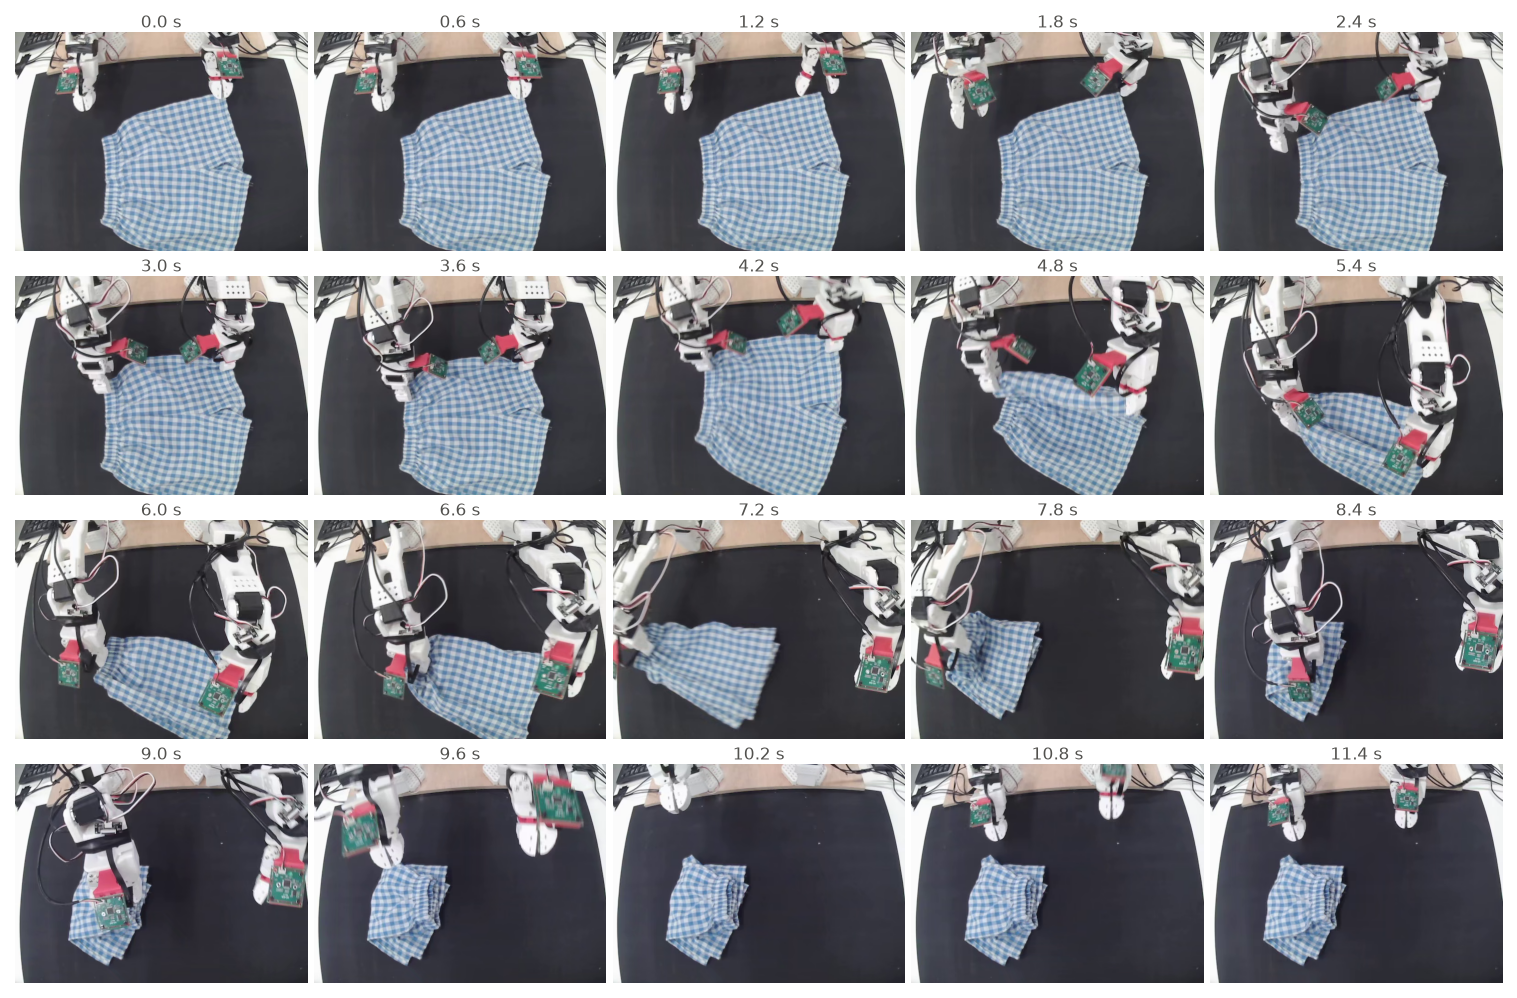
\includegraphics[width=0.78\textwidth]{trajectory_strip.png}
  \caption{\new{One held-out demonstration seen by the overhead camera, 20
  frames evenly spaced from start to end. The arms grasp the waistband, fold
  the shorts over and release.}}
  \label{fig:trajectory}
\end{figure}

We train every model on the first 58 demonstrations and test it on the
\emph{last seven}, which it never sees. \new{The last seven were recorded at
the end of the session. If something changed slowly during the session, such
as the lighting or wear on the gels, the test set would differ from the
training set for that reason alone. To check this, we retrain ACT and
Diffusion on a \emph{random seven} held out from across the whole session.
Section~\ref{sec:compare} compares the two.}

\subsection{How we measure}
\label{sec:measures}

\textbf{Action error.} We give a model one observation and compare the chunk it
plans with the commands the demonstrator actually sent next. We take the
root-mean-square error (RMSE) over all twelve joints, in degrees, separately for
each step of the chunk. We sample one frame in twenty, which gives 1127 scored
frames from the training demonstrations and 111 from the test demonstrations.
Models plan different distances ahead, and error grows with distance, so we
compare models over the first ten steps (\SI{0.33}{\second}), which every model
plans. The \emph{gap} is the test error divided by the training error. Models
that sample have their random seed fixed, so a score repeats exactly.

\begin{newtext}
\textbf{Grad-CAM} \citep{selvaraju2017gradcam} shows where in an image a
model's output comes from. We take the magnitude of the planned chunk as the
output. We then compute its gradient with respect to the last feature map of
the ResNet encoder, average that gradient over each channel to get one weight
per channel, and sum the channels with these weights. Negative values are set
to zero, and the map is scaled so its peak is one and enlarged to the image
size. Grad-CAM needs a convolutional feature map, so it applies to ACT and
Diffusion but not to pi0.5.

\textbf{Input contribution.} To ask how much a model uses one input, we replace
that input with an uninformative version and measure how far the plan moves.
An image is replaced by a flat image of its own average colour, which keeps its
brightness but removes all structure. The joint positions are replaced by a
constant. The distance between the two plans is the mean, over the chunk, of the
Euclidean distance between their commands. We do this for each input in turn
and divide each distance by their sum, so the contributions of one model add up
to 100\,\%. Because they are normalised within a model, the percentages rank a
model's inputs; they cannot be compared in size between models. For models
that sample, the seed is fixed during this, since otherwise sampling noise
alone moves the plan by far more than removing a camera does.

\textbf{World models.} We score frames in two ways. \emph{Reconstruction}
passes frames the model has already seen through its own image autoencoder and
back. \emph{Prediction} compares the frames the model generates for the future,
together with its own planned actions, with what the cameras actually recorded.
Both use peak signal-to-noise ratio (PSNR, in decibels, higher is better) and
the structural similarity index (SSIM, from 0 to 1). We score every sensor
separately. As a baseline we repeat the last frame the model saw; a model that
cannot beat this has learned nothing about how the scene moves.
\end{newtext}

\subsection{The tactile crop}
\label{sec:cropmethod}

\begin{newtext}
Our earlier Grad-CAM pictures showed ACT putting weight near the edges of the
tactile images before contact. Figure~\ref{fig:rimevidence} measures what the
images themselves show before contact. On each sensor the brightest edge is 10 to
21\,\% brighter than the centre, which fits light leaking in at the gel boundary. However, the
brightest feature on every sensor is a vertical ridge inside the gel, about a
third of the way across, not the edge. So the images support a brighter rim,
but they do not show that the rim is the strongest signal before contact.
\end{newtext}

\begin{figure}[t]
  \centering
  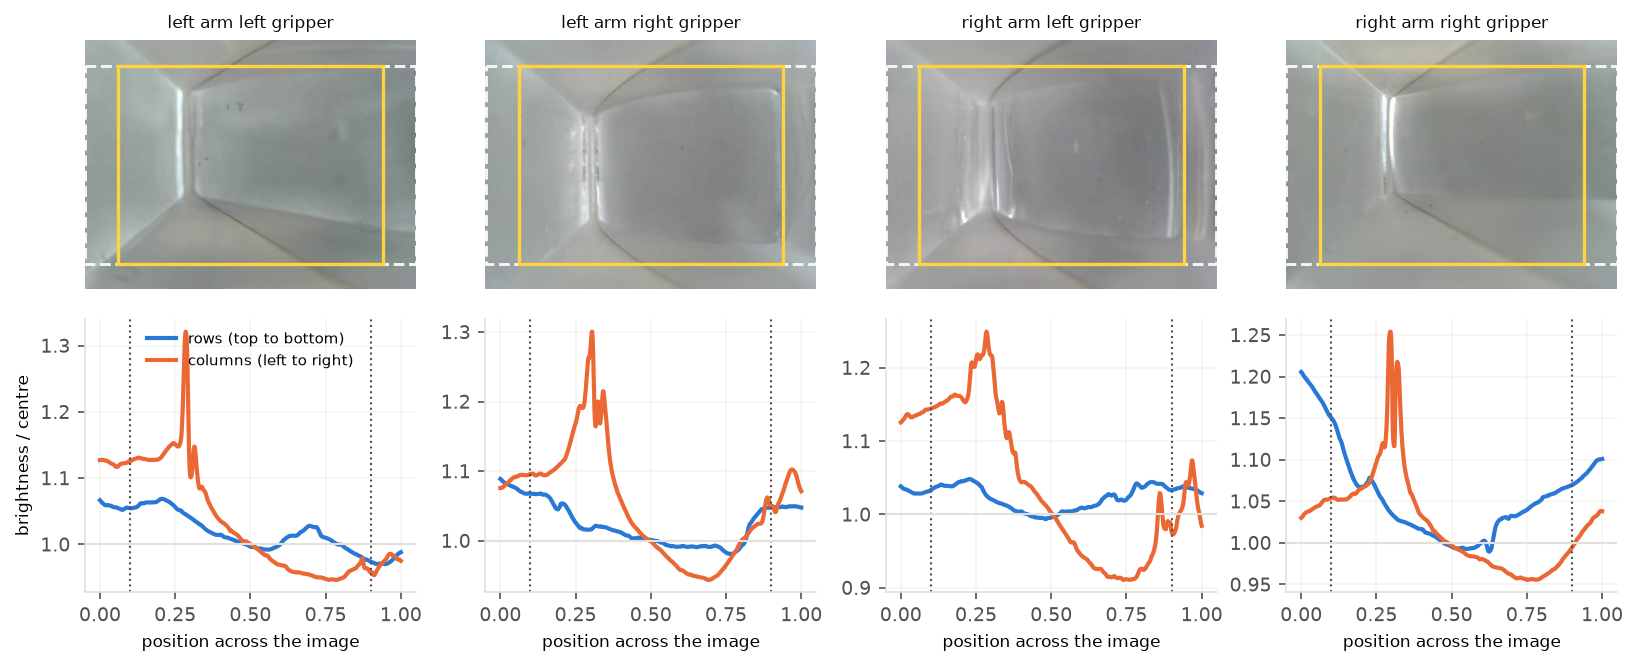
\includegraphics[width=0.92\textwidth]{rim_evidence.png}
  \caption{\new{The four fingertip sensors before contact. Top: the first frame
  of one demonstration, with the rows-only crop (dashed) and the four-edge crop
  (solid). Bottom: brightness of each row and column relative to the centre of
  the gel, averaged over the first frame of all 65 demonstrations; dotted lines
  mark the crop boundaries. The sharp peak in the columns is a ridge in the gel,
  not the rim.}}
  \label{fig:rimevidence}
\end{figure}

We test three crops, each applied to all four fingertip images. \emph{Rows
only} removes the top and bottom tenth of the image. We measured beforehand
that the columns carry contact signal right up to the edge on two sensors,
while every sensor has spare rows. \new{\emph{Four edges} removes a tenth from
every side.} Both then resize the image back to its original shape, which
stretches it. \emph{Rows without stretching} keeps the cropped image at its
smaller size. Only ACT accepts cameras of different sizes, so only ACT gets
this third crop. \new{The crop is part of the model's saved input pipeline, so
it is applied during training and again at test time. We confirmed this in the
saved pipeline of every cropped model.} Apart from the crop, a cropped model is
identical to its uncropped version: the same architecture, data, number of
steps, batch size and random seed.

\section{Experiments}
\label{sec:experiments}

We report four experiments, in the order of the questions in
Section~\ref{sec:intro}. Section~\ref{sec:compare} compares all the models,
Section~\ref{sec:crop} tests the tactile crop, Section~\ref{sec:sensors} asks
which sensors ACT needs \new{and which inputs each model uses}, and
Section~\ref{sec:wm} scores the world action models' predictions of the
cameras.

\subsection{Comparing the models}
\label{sec:compare}

Table~\ref{tab:actions} gives every model's action error on the training and
test demonstrations, and Figure~\ref{fig:horizon} shows how the error grows
with how far ahead the model plans.

\begin{table}[t]
  \centering
  \caption{Action error (RMSE, degrees) on the 58 training and the 7 test
  demonstrations. The left block scores each model over its own plan; the
  right block scores every model over the first ten steps
  (\SI{0.33}{\second}), the only block that is fair across rows. \emph{Gap} is
  test error divided by training error. \new{The lowest error in each column is
  in bold.}}
  \label{tab:actions}
  \small
  \begin{tabular}{lrrrrrr}
\toprule
& & \multicolumn{3}{c}{over its own plan} & \multicolumn{2}{c}{over the first 10 steps} \\
\cmidrule(lr){3-5}\cmidrule(lr){6-7}
model & plan & train & test & gap & test & gap \\
\midrule
ACT & 100 & 2.67 & 14.09 & 5.3 & 7.88 & 3.4 \\
Diffusion & 32 & 4.74 & 9.18 & 1.9 & 5.03 & 2.8 \\
pi0.5 & 50 & 17.05 & 18.35 & 1.1 & 8.96 & 1.1 \\
pi0.5, three passes & -- & -- & -- & -- & -- & -- \\
Flow matching & 50 & 7.57 & 14.44 & 1.9 & 4.51 & 1.4 \\
DreamZero & 24 & \textbf{0.94} & 7.02 & 7.4 & 4.17 & 5.3 \\
FastWAM & 10 & 1.53 & \textbf{3.94} & 2.6 & \textbf{3.94} & 2.6 \\
\bottomrule
\end{tabular}

\end{table}

\begin{figure}[t]
  \centering
  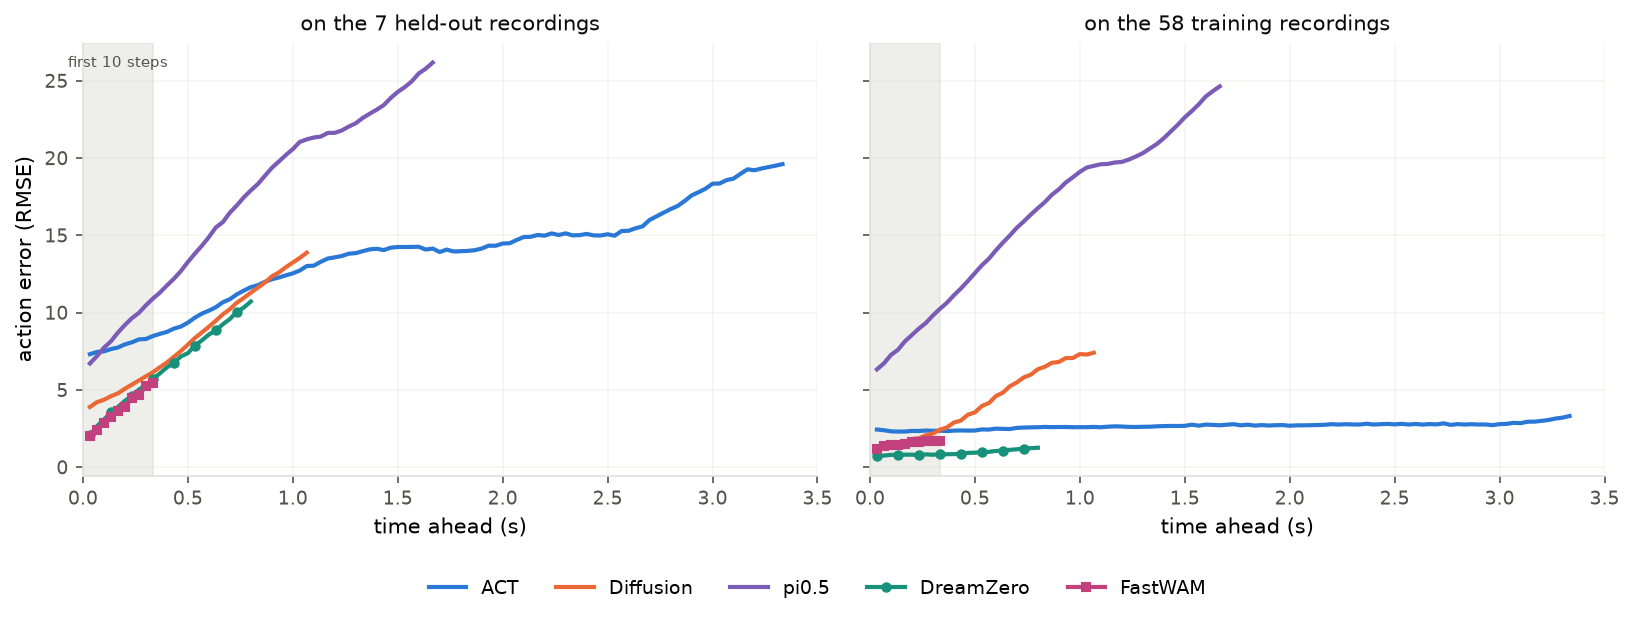
\includegraphics[width=0.72\textwidth]{horizon_all.png}
  \caption{Action error at each step of the plan, against how far ahead that
  step is, for every model on one linear scale. Left: test demonstrations.
  Right: training demonstrations. The shaded band is the first ten steps, which
  every model plans.}
  \label{fig:horizon}
\end{figure}

\textbf{Both world action models plan the next ten steps better than every
other model on unseen demonstrations.} Over those steps their test errors are
3.9 (FastWAM) and 4.2 (DreamZero). The two are too close to rank. Their lead is
several times larger than the change we see when we rerun them with different
random seeds (Appendix Table~\ref{tab:floor}). It does not prove that
predicting the future is what helps: FastWAM starts from a pretrained video
model, and DreamZero \new{is given the past \SI{1.6}{\second} of arm commands}.

\rev{\textbf{Flow matching is the most accurate behaviour-cloning policy}, over
the first ten steps and further ahead: 4.3 against Diffusion's 5.0 over ten
steps, 7.3 against 7.6 over 24 and 9.0 against 9.2 over 32. Flow matching and
pi0.5 share their training objective, and flow matching's error over the first
ten steps is half pi0.5's (4.3 against 9.0). On our data, pi0.5's pretraining
with our narrow LoRA does worse than training a small model from scratch. Our
first flow-matching run saw only a random \(84\times84\) patch of each camera
image, about 2\,\% of it (Section~\ref{sec:models}), and 98.7\,\% of what moved
its plan was proprioception. Retrained on whole,
resized images, it improves on the test demonstrations from 14.4 to 11.5 over
its plan, but only from 4.5 to 4.3 over the first ten steps. Over a third of a
second the arms' own positions predict the next commands almost entirely;
seeing the cameras matters further ahead.}

\textbf{Diffusion's error starts low but grows fastest.} On the test
demonstrations it rises from 3.9 at the first step to 13.9 by step 32, a factor
of 3.6; ACT starts at 7.3 but grows by only 1.8, so the two cross at about one
second (Figure~\ref{fig:horizon}). On the training demonstrations ACT's error is
almost flat over all 100 steps (2.4 to 3.3): it replays a familiar
demonstration almost exactly.

\textbf{Every model is much worse on unseen demonstrations.} ACT's error is
about five times higher on the test demonstrations than on the training ones,
and Diffusion's about twice as high. \new{Because the last seven demonstrations
are also the latest, a slow change over the afternoon could make them harder.
When the seven are instead picked at random, each sits between training
demonstrations in time, so drift should make them easier; the gap grows instead
(8.9 against 5.3 for ACT, 2.6 against 1.9 for Diffusion; Appendix
Figure~\ref{fig:split}). Drift does not explain the gap.}

\textbf{pi0.5's small gap does not mean it generalises well.} Its error on
the demonstrations it trained on is already higher than Diffusion's on
demonstrations it never saw: after about one pass over the data, adapting only
the small LoRA addition, it never fitted the training set. \new{Trained for
about three passes (\num{70000} steps), it barely moved: training error fell
from 17.1 to 16.4 and test error from 18.4 to 18.0, less than rescoring with
another seed moves it (Appendix Table~\ref{tab:floor}). The narrow LoRA, not
too little training, is the likelier limit.}

\rev{\subsection{Do the test demonstrations look different?}
\label{sec:recordings}

Figure~\ref{fig:recordings} shows how far apart every pair of the 65
demonstrations looks to each model's own vision encoder
(Section~\ref{sec:measures}), and Table~\ref{tab:recordings} asks the question
that matters for the gap above: is a test demonstration further from its
nearest training demonstration than a training demonstration is from its
nearest neighbour?

\begin{figure}[t]
  \centering
  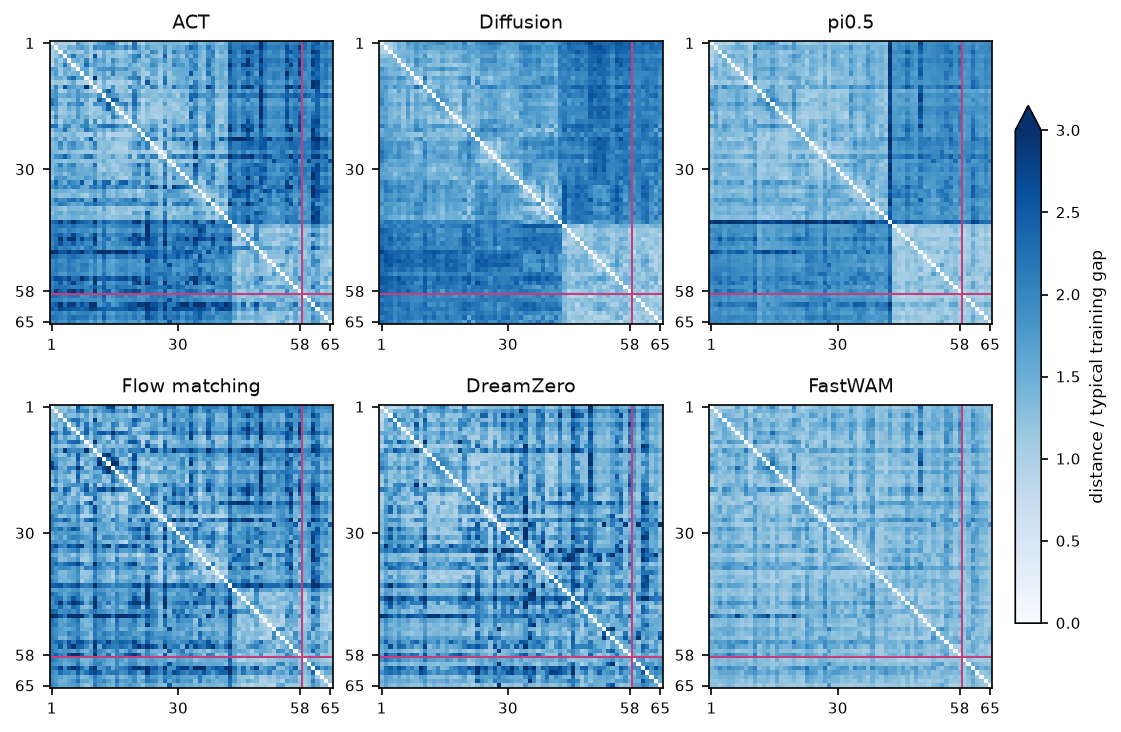
\includegraphics[width=0.85\textwidth]{recordings.png}
  \caption{How different every pair of demonstrations looks to each model's
  vision encoder: the mean feature distance after matching their frames in
  order, scaled so that 1 is the most different pair. Demonstrations are in
  recording order; the lines mark the seven test demonstrations (58--65).}
  \label{fig:recordings}
\end{figure}

\begin{table}[t]
  \centering
  \caption{Distance from each demonstration to its nearest training
  demonstration (itself excluded), averaged over the 58 training and the 7 test
  demonstrations, on the scale of Figure~\ref{fig:recordings}.}
  \label{tab:recordings}
  \small
  \begin{tabular}{lrrr}
\toprule
model & training & test & test / training \\
\midrule
ACT & 0.26 & 0.28 & 1.07 \\
Diffusion & 0.36 & 0.32 & 0.90 \\
pi0.5 & 0.30 & 0.29 & 0.96 \\
Flow matching & 0.23 & 0.24 & 1.05 \\
DreamZero & 0.26 & 0.30 & 1.16 \\
FastWAM & 0.32 & 0.35 & 1.07 \\
\bottomrule
\end{tabular}

\end{table}

\textbf{To every model, the test demonstrations look like training ones.} A
test demonstration is between 0.90 and 1.16 times as far from its nearest
training demonstration as a training demonstration is from its own nearest
neighbour (Table~\ref{tab:recordings}). Each test demonstration has training
demonstrations that look about as similar as training demonstrations look to
each other, so the large gaps of Section~\ref{sec:compare} are not caused by
the test demonstrations looking unfamiliar.

\textbf{The session does contain one visual change, at demonstration 43.} ACT,
Diffusion and pi0.5 split the session into two blocks
(Figure~\ref{fig:recordings}). Splitting each encoder's features by camera
puts the boundary in the left arm's left fingertip (LLG) between demonstrations
42 and 43, for ACT, Diffusion, flow matching and pi0.5 alike; no other camera
changes at a common point. The untouched gel's image shows why: between those
two demonstrations the sensor's view shifted, moving the ridge and the pad's
edges and adding new marks on the gel (Appendix Figure~\ref{fig:sensorshift}).
The shift is a step, not a drift: every demonstration before it looks like the
earlier ones and every one after it like the later ones. It does not separate
test from training, since 15 training demonstrations (43--57) come after it
too. DreamZero and FastWAM barely show it, probably because our features for
them average each fingertip onto about four cells of the autoencoder's latent,
too coarse to see the ridge move.}

\rev{\subsection{Learning curves}
\label{sec:curves}

Figure~\ref{fig:curves} follows each model's training and test error over the
first ten steps through training (Section~\ref{sec:measures}). The last point
of each curve reproduces the model's row of Table~\ref{tab:actions} to within
what a rerun moves it: the curves come from fresh runs with the same settings,
and ACT's last point over the first ten steps is 8.7 against 7.9 in the table.

\begin{figure}[t]
  \centering
  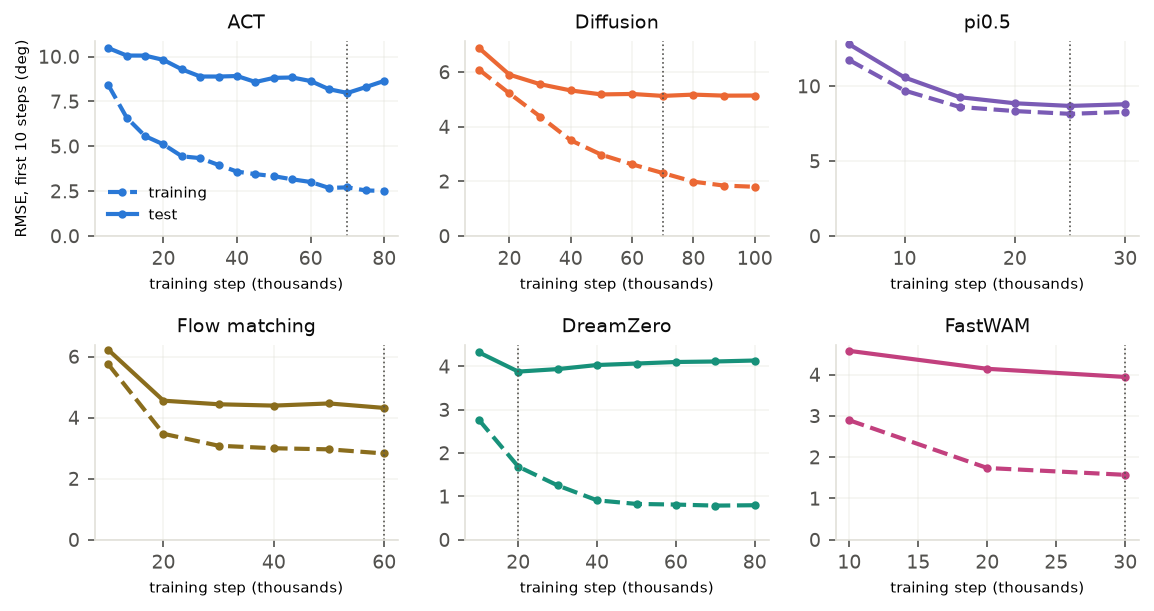
\includegraphics[width=0.85\textwidth]{curves.png}
  \caption{Action error over the first ten steps on the training (dashed) and
  test (solid) demonstrations, at every saved checkpoint of a rerun with the
  same settings. The dotted line marks the checkpoint with the lowest test
  error.}
  \label{fig:curves}
\end{figure}

\textbf{The test error stops improving long before training ends; the training
error does not.} Diffusion's test error levels off at about 5.2 by
\num{40000} of its \num{100000} steps, while its training error keeps falling,
from 3.5 to 1.8. Flow matching's levels off by \num{20000} of \num{60000}.
ACT's training error falls from 8.4 to 2.5 over the whole run, while its test
error moves only from 10.5 to about 8, and over its whole plan not at all (14.7
at \num{5000} steps, 14.3 at the end). The large gaps of
Table~\ref{tab:actions} are therefore built late in training: the extra steps
fit the training demonstrations more closely without helping on new ones.
They do not make the test error worse either, so stopping earlier would save
time, not improve the models.

\textbf{pi0.5 never pulls apart.} Its training and test errors fall together
and level off at about \num{20000} steps, with a gap of 1.1 throughout: it
stops learning rather than overfitting, as Section~\ref{sec:compare} found.

\textbf{The trainer's own held-out loss would have misled us.} LeRobot also
reports each model's training loss on the test demonstrations. For Diffusion
it rises fourfold from \num{10000} steps (0.029 to 0.119), and for flow
matching it rises too, which reads as severe overfitting, yet neither model's
test action error gets worse. These losses score how well a model removes
noise from the recorded actions, not how close its plan is to them.
\pending{DreamZero and FastWAM learning curves.}}

\subsection{Cropping the tactile images}
\label{sec:crop}

Table~\ref{tab:crop} gives the test error of every model with and without each
crop.

\begin{table}[t]
  \centering
  \caption{Test action error (RMSE over each model's own plan) with each
  tactile crop (Section~\ref{sec:cropmethod}). \emph{Rows, unstretched} exists
  for ACT only. Each entry is one training run; \new{the lowest in each row is in
  bold.}}
  \label{tab:crop}
  \small
  \begin{tabular}{lrrrr}
\toprule
model & no crop & rows & rows, unstretched & four edges \\
\midrule
ACT & 14.09 & 14.68 & 14.08 & -- \\
Diffusion & 9.18 & 9.21 & n/a & -- \\
pi0.5 & 18.35 & 18.11 & n/a & -- \\
DreamZero & 7.02 & n/a & n/a & -- \\
FastWAM & 3.94 & n/a & n/a & -- \\
\bottomrule
\end{tabular}

\end{table}

\textbf{Cropping the tactile images changes almost nothing.} With the rows-only
crop, ACT, Diffusion and pi0.5 move by a few per cent at most, in both
directions. That is within what repeating a run with another random seed moves
Diffusion and pi0.5 (Appendix Table~\ref{tab:floor}). \new{The four-edge crop
leaves pi0.5 and Diffusion unchanged (18.34 against 18.35, 9.10 against 9.18)
and costs ACT as much as the rows-only crop does (14.70 against 14.68 and 14.09
uncropped).} \rev{FastWAM's four-edge crop leaves it unchanged too (3.99
against 3.94). The ridge crop, which also removes the gel's bright ridge, is no
different: pi0.5 18.49, Diffusion 9.06 and ACT 14.63, again within a few per
cent of uncropped and, for ACT, the same cost as its other crops. DreamZero's
ridge crop leaves it unchanged as well (6.98 against 7.02).}
\pending{DreamZero's four-edge crop and FastWAM's ridge crop.} For ACT, the one place the rows-only crop looked
harmful, over the far end of its plan, disappears when the image is not
stretched. So the stretching, not the loss of the rim, caused that small
penalty.

\textbf{The policies do not over-weight the edges of the tactile images.}
Appendix Figure~\ref{fig:rim} measures this directly with Grad-CAM. A value of 1 means the edge band
gets exactly its share of the weight by area; above 1, the model favours the
edge. On a test demonstration, every uncropped model sits between two thirds
and nine tenths of its share, at every band width. \new{So the strong edge
weighting of Figure~\ref{fig:gradcamevidence} happens at some moments but does
not hold on average.} Cropping moves the weight slightly towards the new edge,
partly for a mechanical reason: after cropping and stretching, the pixels
nearest the edge used to be further in.

\begin{figure}[t]
  \centering
  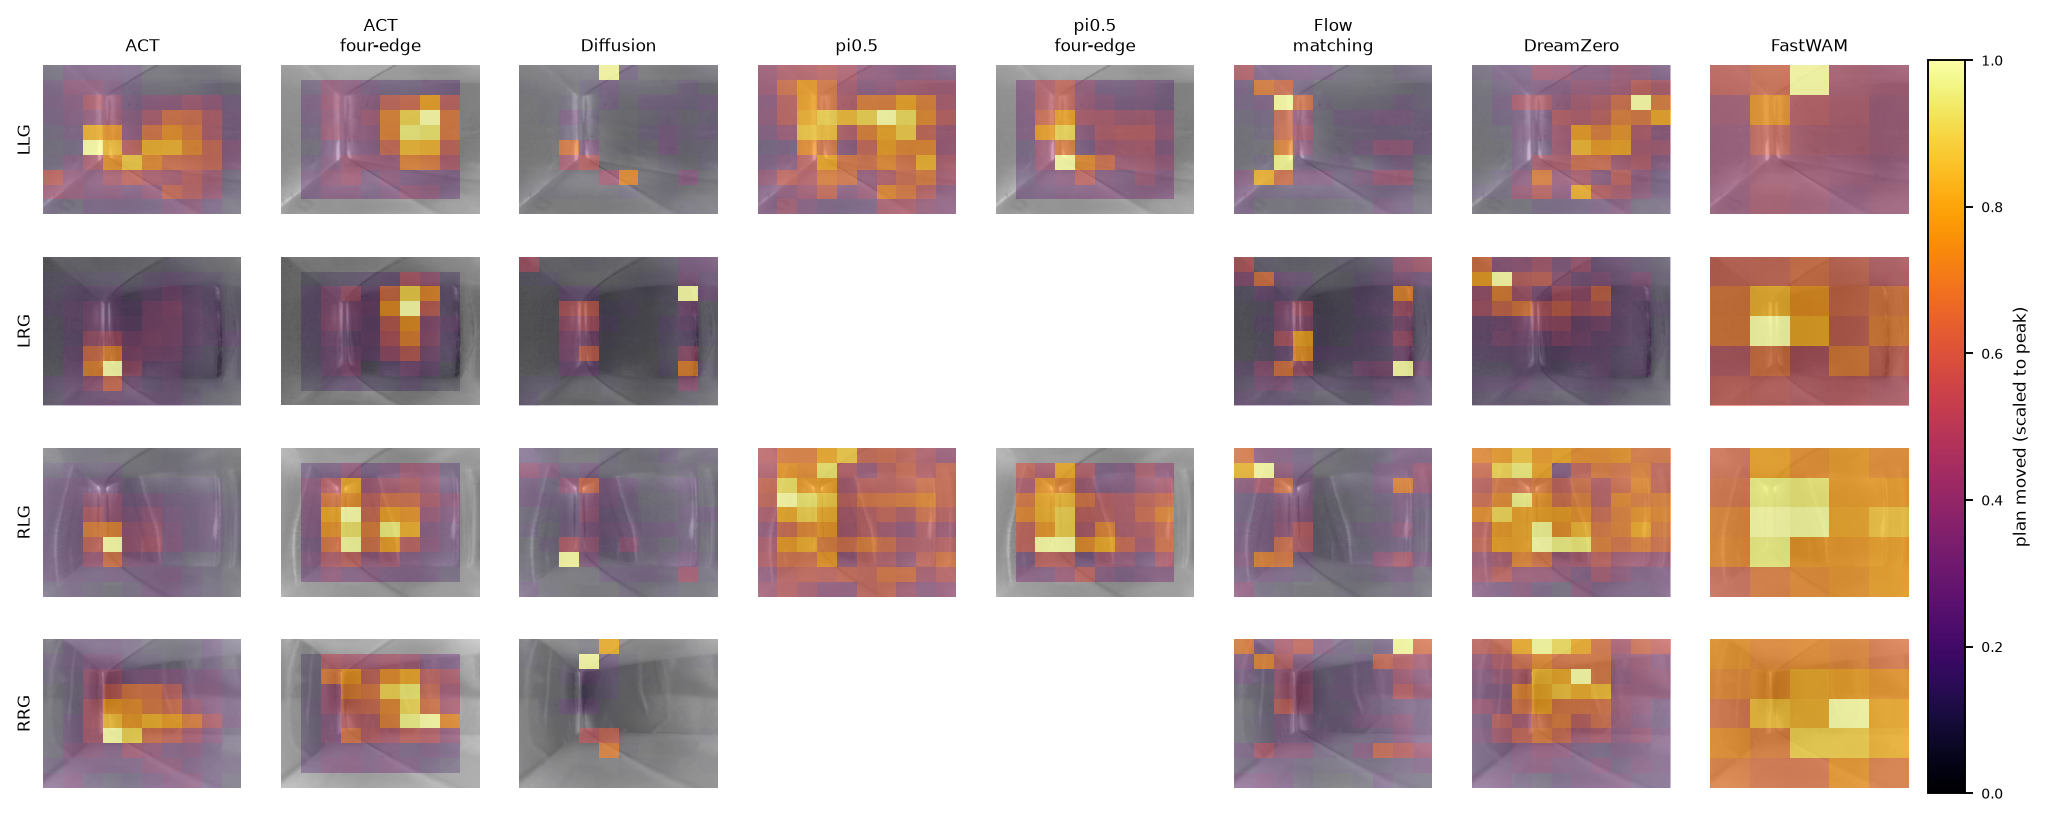
\includegraphics[width=0.6\textwidth]{patch_maps.png}
  \caption{\new{Patch occlusion maps: where in each fingertip image the plan
  comes from, averaged over 20 to 60 frames of test demonstration 58 (FastWAM:
  8 frames, $5\times5$ cells per sensor). Darker cells moved the plan more when
  painted over; each map is scaled to its own peak. A cropped model's map is
  drawn over the full image, so the white border is what it never sees. pi0.5
  reads only LLG and RLG.}}
  \label{fig:patchmaps}
\end{figure}

\new{\textbf{Cropping moves ACT's attention off the ridge; pi0.5's stays on it.}
Figure~\ref{fig:patchmaps} answers the question for models Grad-CAM cannot
reach, using patch occlusion. On each sensor we locate the five cells that move
the plan most. For uncropped ACT they sit 0.31 to 0.47 of the way across, around
the gel's ridge at about 0.3, and the outer fifth of the image gets 0.68 of its
share by area, in line with Grad-CAM. With the four-edge crop they move to 0.45
to 0.69, the right half of the gel, where the contact marks form. pi0.5 with the
four-edge crop still peaks at 0.33 to 0.35, on the ridge, which is what the
ridge crop removes. FastWAM's map is nearly flat: painting any cell moves its plan by at
least 40\,\% as much as the most important cell. Its pinned plan repeats
exactly, so this is the model and not sampling noise: it reacts to a change
anywhere in a fingertip image by about the same amount.}
\rev{Uncropped Diffusion peaks 0.37 to 0.53 across, just right of the ridge;
uncropped pi0.5 peaks in different places on its two sensors (0.61 and 0.23)
and its maps are flatter than the behaviour-cloning policies'; DreamZero's
peaks are scattered (0.13 to 0.73), and retrained flow matching's lie between
0.21 and 0.55. \textbf{No model over-weights the image edges:} the outer fifth
of the image gets 0.78 (Diffusion), 0.88 (DreamZero), 0.91 (pi0.5) and 0.95
(flow matching) of its share by area, all below one. Uncropped ACT, at 0.68, is
the most centred.}

\subsection{Which sensors the models use}
\label{sec:sensors}

We retrained ACT with three sets of inputs, all with proprioception: the
overhead camera alone; the overhead camera and one fingertip per arm (the pair
pi0.5 reads); and all five cameras. Table~\ref{tab:sensors} gives the result.
\new{The overhead-only model tests the reading of Appendix Figure~\ref{fig:framewise}: if
ACT uses touch only briefly, removing touch altogether should cost little.}

\begin{table}[t]
  \centering
  \caption{ACT trained on three sets of cameras, all with proprioception.
  Action error (RMSE) over its own 100-step plan and over the first ten steps.
  \new{The lowest error in each column is in bold.}}
  \label{tab:sensors}
  \small
  \begin{tabular}{lrrrrr}
\toprule
& \multicolumn{3}{c}{over its 100-step plan} & \multicolumn{2}{c}{first 10 steps} \\
\cmidrule(lr){2-4}\cmidrule(lr){5-6}
cameras & train & test & gap & test & gap \\
\midrule
overhead & -- & -- & -- & -- & -- \\
overhead + one fingertip per arm & -- & -- & -- & -- & -- \\
overhead + all four fingertips & 2.67 & 14.09 & 5.3 & 7.88 & 3.4 \\
\bottomrule
\end{tabular}

\end{table}

\new{\textbf{ACT generalises better without the fingertips.} Trained on the
overhead camera alone, it fits its training demonstrations exactly as well as
with all five cameras (2.62 against 2.67), but its test error is lower: 13.8
against 14.1 over its plan, and 5.8 against 7.9 over the first ten steps. So on
new demonstrations the fingertips do not help ACT, and may hurt it. Each setting
is one training run, and we have not measured how much a second run with
another seed would move these numbers (Appendix~\ref{sec:threats}).
Adding one fingertip per arm back does not help either: 14.8 over the plan and
7.5 over the first ten steps, between the other two. Neither tactile set beats
the overhead camera alone.}

\begin{figure}[t]
  \centering
  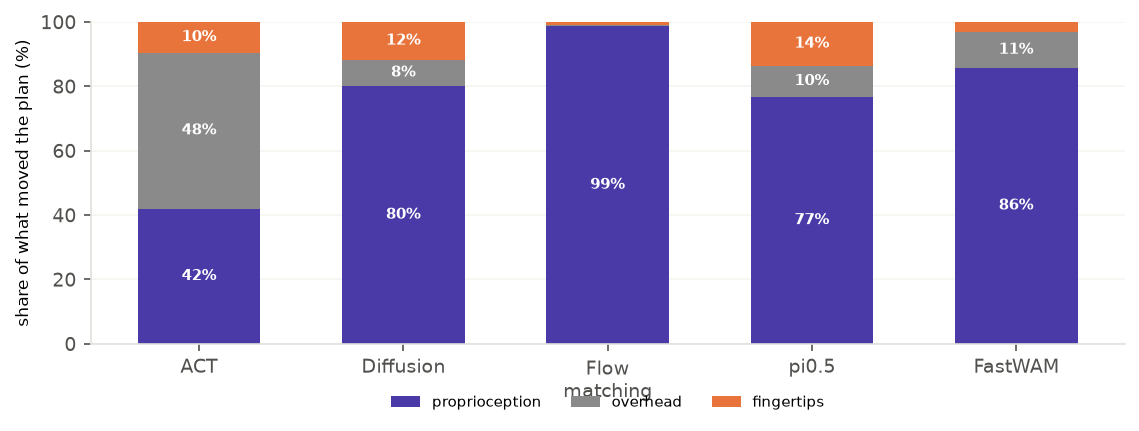
\includegraphics[width=0.5\textwidth]{stream_shares.png}
  \caption{How much each input moves each model's plan (input contribution,
  Section~\ref{sec:measures}). Each bar adds up to 100\,\%, so compare the
  order of inputs within a bar, not heights between bars. pi0.5 reads two
  fingertips; the others read four. \rev{DreamZero alone is given its past
  arm commands as an input.}}
  \label{fig:streams}
\end{figure}

Figure~\ref{fig:streams} shows which inputs the policies actually use. ACT
relies most on the overhead camera, then proprioception, with the fingertips
last. Diffusion and pi0.5 rely mostly on proprioception: about three quarters
of what moves pi0.5's plan is where the arms are. \new{FastWAM leans on
proprioception most of all, 86\,\%, with 11\,\% for the overhead camera and
3\,\% for the fingertips.} \rev{Retrained on whole images, flow matching
uses its cameras: proprioception falls to 75\,\% (98.7\,\% in the first run),
with 9\,\% for the overhead camera and 16\,\% for the fingertips, the largest
fingertip share of any model. DreamZero leans on proprioception most of all
(88\,\%), then on its past commands (10\,\%); all five cameras together move
its plan by only 2.3\,\%. The model that plans the next ten steps second best
barely reads its cameras to do it.}


\subsection{How well the world action models predict the cameras}
\label{sec:wm}

Table~\ref{tab:wm} scores both world action models on every sensor. The first
column is reconstruction, the frames the model saw passed through its own
autoencoder, which is the sharpest any of its predictions can be. \new{For
DreamZero this is its frozen image autoencoder, applied to each frame; for
FastWAM it is Wan2.2's video autoencoder, which compresses groups of four
frames together.} The next columns compare its predicted future frames with the
real ones and with repeating the last frame it saw.

\begin{table}[t]
  \centering
  \caption{World action models on the seven test demonstrations, per sensor, in
  PSNR (dB, higher is better). \emph{Reconstruction}: seen frames through the
  model's own autoencoder. \emph{Prediction}: predicted future frames.
  \new{\emph{Repeat last}: the last seen frame used as the prediction for every
  future time.} Both averaged over the prediction horizon. \emph{Margin}:
  prediction minus repeat last, at \SI{0.8}{\second} ahead and at the end of
  each model's horizon (\SI{4.8}{\second} for DreamZero, \SI{1.1}{\second} for
  FastWAM). Each model works at its own resolution, so compare margins, not
  PSNR, between models.}
  \label{tab:wm}
  \small
  \begin{tabular}{llrrrrr}
\toprule
& & & & & \multicolumn{2}{c}{margin} \\
\cmidrule(lr){6-7}
sensor & model & reconstruction & prediction & repeat last & at \SI{0.8}{\second} & at end \\
\midrule
overhead & DreamZero & 17.3 & 15.5 & 14.1 & -4.1 & +3.2 \\
LLG & DreamZero & 37.0 & 30.1 & 25.9 & -1.3 & +5.6 \\
LRG & DreamZero & 34.9 & 28.0 & 22.9 & -1.4 & +6.7 \\
RLG & DreamZero & 33.9 & 24.8 & 20.7 & +0.0 & +5.0 \\
RRG & DreamZero & 37.0 & 26.8 & 23.6 & +1.5 & +2.6 \\
overhead & FastWAM & 33.8 & 18.5 & 18.6 & +0.2 & +0.4 \\
LLG & FastWAM & 46.7 & 33.0 & 32.9 & +5.2 & +5.2 \\
LRG & FastWAM & 46.1 & 31.5 & 33.4 & +2.7 & +4.3 \\
RLG & FastWAM & 45.9 & 28.5 & 26.5 & +5.0 & +6.3 \\
RRG & FastWAM & 47.2 & 30.0 & 29.0 & +3.0 & +3.1 \\
\bottomrule
\end{tabular}

\end{table}

\textbf{Most of the prediction error comes from predicting, not from
compressing the images.} DreamZero's small image autoencoder is the exception
on the overhead camera: it reproduces a seen frame at only 17.3\,dB, and the
model's predictions reach 15.5\,dB, close to that ceiling. \new{(At 17.3\,dB a typical
pixel is off by 14\,\% of the full brightness range, a visibly blurred image;
at 35\,dB it would be off by under 2\,\%.)} On the fingertips its
autoencoder reaches 34 to 37\,dB, but its predictions only 25 to 30\,dB.
FastWAM's pretrained autoencoder is much sharper, 34\,dB on the overhead camera
and about 46\,dB on the fingertips, and its predictions sit 13 to 17\,dB below
that. So a better autoencoder would remove little of either model's error,
except DreamZero's on the overhead camera.

\textbf{DreamZero predicts the cameras better than repeating the last frame,
on every sensor, from \SI{1.6}{\second} ahead onwards.} Its margin is roughly 3
to 8\,dB, and largest on the fingertips, where repeating the last frame is
already strong because the gels change only at contact. At \SI{0.8}{\second} it
only ties, because the future still looks almost exactly like the present.
\new{In Figure~\ref{fig:filmstrip} its reconstruction of the seen frame is
already blurred, but it predicts the arms leaving and the folded shorts staying
where they are, as really happened.}

\textbf{FastWAM predicts sharp frames, but a frame-averaged score barely
rewards them.} It predicts only about a second ahead. On the overhead camera it
ties with repeating the last frame, although its frames move the grippers in
the right direction (Figure~\ref{fig:filmstrip}). \new{Its difference row
shows the error concentrated on the moving arms and cloth, where its motion lags
the real one; everywhere else it is flat grey.} The garment fills most of the
frame and hardly moves within a second, so repeating the last frame is already
right about most pixels. \textbf{A score averaged over the
whole frame can rate a correct prediction of a small moving part as no better
than doing nothing.} On the fingertips, where contact changes many pixels,
FastWAM starts below repeating the last frame and ends 3 to 6\,dB above it on
every sensor. At the one moment both models predict, \SI{0.8}{\second} ahead,
FastWAM is ahead on both panels of Appendix Figure~\ref{fig:predmargin}.

\begin{figure}[t]
  \centering
  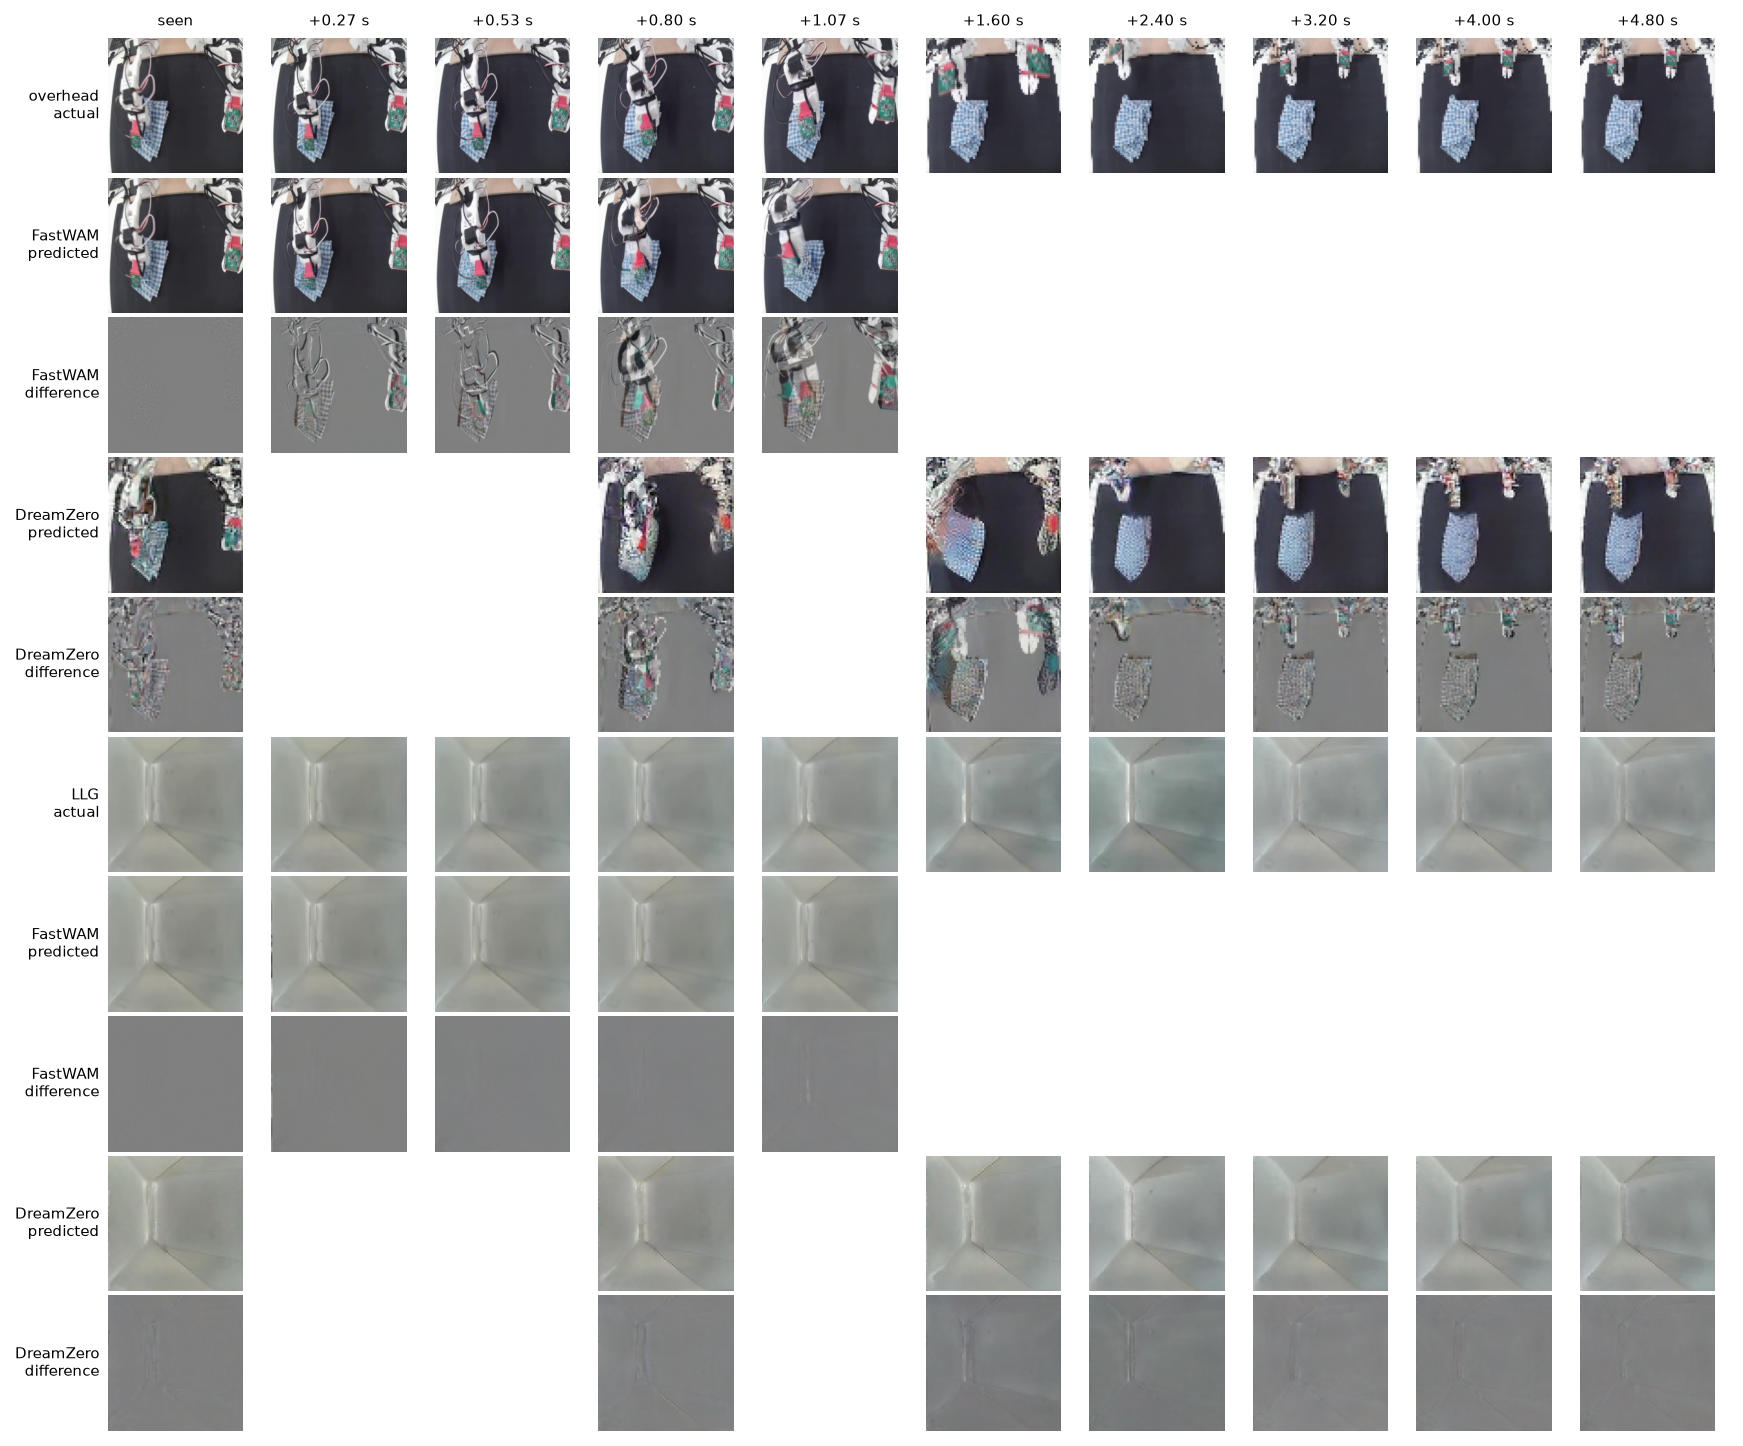
\includegraphics[width=0.6\textwidth]{filmstrip_h2h.png}
  \caption{\new{FastWAM and DreamZero predicting from the same seen frame
  (test demonstration 58, 8\,s in, as the arms release the folded shorts), on
  one time axis. For the overhead camera and one fingertip (LLG) the rows are
  what happened, each model's prediction, and its difference from what happened
  (truth minus prediction, rescaled so that mid-grey is no error). The
  \emph{seen} column shows each model's reconstruction of the frame it was
  given. Blank cells are times a model does not predict. Each model is shown at
  its own resolution. Appendix Figure~\ref{fig:filmstripearly} shows an earlier
  moment.}}
  \label{fig:filmstrip}
\end{figure}

\rev{\subsection{Does FastWAM's touch prediction follow the gripper?}
\label{sec:grasp}

We scored FastWAM's fingertip predictions over the 36 grasps of the test
demonstrations (35 distinct windows, since two grasps start on the same frame),
on the two fingertips of the grasping arm. Table~\ref{tab:grasp} gives the mean
absolute pixel error as a percentage of the pixel range, and
Figure~\ref{fig:grasp} shows one grasp.

\begin{table}[t]
  \centering
  \caption{FastWAM around the 36 test grasps: mean absolute pixel error (\% of
  the pixel range) of the grasping arm's two fingertips, over the eight
  predicted frames. \emph{Change from recorded} is how far the prediction moves
  when the current gripper position given to the model is changed from the
  recorded (open) value to closed. \emph{Repeat-last error} is the error of
  repeating the seen frame, which is also how much the gel really changes.}
  \label{tab:grasp}
  \small
  \begin{tabular}{lrrr}
\toprule
condition & error & change from recorded & repeat-last error \\
\midrule
recorded & 5.44 & 0.00 & 8.00 \\
closed & 5.47 & 1.38 & 8.00 \\
\bottomrule
\end{tabular}

\end{table}

\begin{figure}[t]
  \centering
  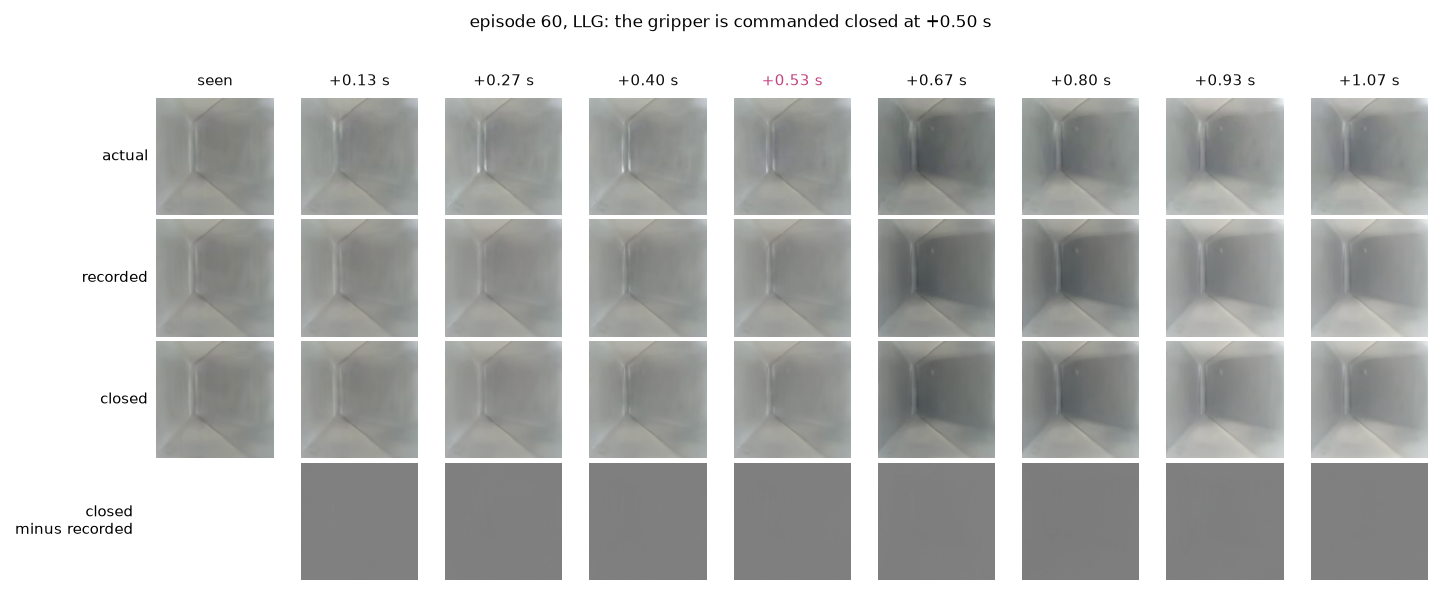
\includegraphics[width=\textwidth]{grasp_filmstrip_state.png}
  \caption{One grasp (test demonstration 60, left arm, fingertip LLG). Rows:
  what happened; FastWAM's prediction with the recorded gripper position;
  its prediction when told the gripper is already closed; and the difference
  between the two predictions (mid-grey is none). The \emph{seen} column shows
  the model's reconstruction of the frame it was given. The gripper is
  commanded closed at \SI{0.5}{\second}; the gel darkens at contact about a
  tenth of a second later.}
  \label{fig:grasp}
\end{figure}

\textbf{FastWAM predicts the contact, and when it happens, from the image it
sees.} In Figure~\ref{fig:grasp} it darkens the gel at the same moment the real
gel darkens, about a tenth of a second after the closing command, and it never
saw that command. Over all 36 grasps its error (5.4\,\%) is a third lower than
repeating the seen frame (8.0\,\%).

\textbf{Telling it the gripper is already closed changes almost nothing.} The
prediction moves by 1.4\,\% when the gripper position is set to closed, against
8.0\,\% of real change in the gel, and its error is the same (5.5\,\%). The
difference row of Figure~\ref{fig:grasp} is flat grey. FastWAM reads the
coming grasp from the images (where the arm is, where the cloth is), not from
the gripper's position. \pending{the FastWAM whose video reads the actions,
with the grasp commanded and with the gripper held open.}}

\section{Discussion}
\label{sec:discussion}

\textbf{What we learned.} The largest effect in this report is not a difference
between models. It is the drop from training to unseen demonstrations, which
every model shows and which is not caused by drift over the session. \rev{Nor is
it caused by the test demonstrations looking unfamiliar, and it is built late in
training: for all but FastWAM, test error levels off early while training error
keeps falling.}
Fifty-eight demonstrations of one task from one session are not enough for any
of these models to generalise to a fifty-ninth.

Cropping the tactile images is not the lever. It changes almost nothing on any
model, and \rev{no model} over-weights the image edges that motivated it.
\new{Pretraining did not help as we used it: pi0.5, finetuned through a narrow
LoRA, plans worse than a small flow-matching policy trained from scratch, and
three times more training did not close the gap.}

Touch is used, but briefly, \new{and removing the fingertips altogether made
ACT slightly better on held-out demonstrations. On a task this consistent, the
overhead camera and the joint positions may already say what the next commands
should be.} The two world action models plan the near future best, though
DreamZero barely reads its cameras to do so.

\textbf{Next steps.} \textbf{Collect more varied demonstrations} (sessions,
garments, starting positions), the most direct attack on the generalisation
gap. \textbf{Test on the robot}, since agreement with recorded commands is not
folding the garment. \new{\textbf{Finetune pi0.5 fully, or with LoRA on every
layer,} as the published recipes do.} \textbf{Score motion, not whole frames}, which frame-averaged PSNR ignores.


\appendix
\rev{\section{Model details}
\label{sec:modeldetails}

\textbf{How pi0.5 is usually adapted.} Its authors finetune the whole model on
each new task; their code also offers LoRA \citep{hu2022lora}, which trains
small low-rank corrections to chosen weights and freezes the rest, applied
there to both the vision-language model and the action expert. On OpenVLA,
LoRA of rank 32 on every linear layer matched full finetuning
\citep{kim2024openvla}; on language models LoRA learns less of a new task,
though it forgets less \citep{biderman2024lora}. Ours (rank 16 on the action
expert's attention and its state and action layers, about 1.3 million trained
weights) is narrower than any of these.

\textbf{How DreamZero is usually adapted.} Its authors adapt it to a new robot
by finetuning the 14-billion-parameter pretrained model on about 30 minutes of
the robot's play data, not by training from scratch. Our 59-million-parameter
version from scratch is therefore a test of the method alone.

\textbf{How FastWAM is usually adapted.} Its authors finetune the pretrained
Wan2.2 video model with its action expert on each task's demonstrations
(\num{20000} to \num{30000} steps), and skip video prediction at test time; we
do the same, starting from the public LeRobot base, and run the video
prediction only to score it.}

\gr{\subsection*{Architectures}

Figure~\ref{fig:arch} draws each model as it runs here, from the inputs it
reads to the chunk it outputs, and Tables~\ref{tab:hyper-bc}
and~\ref{tab:hyper-big} give every setting that differs between them. All six
read the twelve joint positions and are trained on the first 58 demonstrations
with seed 1000; all actions and joint positions are normalised by the training
data's mean and standard deviation (pi0.5: its own quantile normalisation),
and their outputs are un-normalised to degrees before scoring.

\textbf{ACT.} Each camera image ($480\times640$) passes through one shared
ResNet-18, initialised from ImageNet; its last feature map ($15\times20$ cells,
512 channels) becomes one token per cell, so each camera contributes 300
tokens. These, a token for the joint positions and a latent token join a
4-layer transformer encoder ($d=512$, 8 heads); a 1-layer decoder with 100
learned queries outputs the 100-step chunk in one pass. In training a
4-layer encoder over the recorded chunk produces a 32-dimensional latent, a
conditional variational autoencoder trained with an L1 action loss plus a KL
term weighted 10; at test time the latent is zero, so the plan is
deterministic.

\textbf{Diffusion Policy.} Each camera has its own ResNet-18, trained from
scratch, on images resized to $180\times240$; a spatial-softmax layer turns its
feature map into 32 keypoints, so each camera gives a 64-number vector. The last
two frames of every camera and the joint positions condition, through FiLM, a
1-D convolutional U-Net (channels 512, 1024, 2048; kernel 5) that removes noise
from a 64-step action sequence. Training follows DDPM with 100 noise levels
(squared-cosine schedule) and predicts the added noise; at test time all 100
denoising steps run from a fixed seed, and the first 32 steps are executed.

\textbf{Flow matching.} One ResNet-18 with GroupNorm, shared by the five
cameras and trained from scratch, sees each image resized to $180\times240$ and
ends in the same 32-keypoint spatial softmax; a linear layer turns each camera's
keypoints into one token, and the joint positions into another. These six
tokens and the 50 noisy action tokens pass through an 8-layer transformer
($d=512$, 8 heads, pre-norm, GELU) with a time embedding added to every token,
which predicts the flow-matching velocity. Training samples the flow time from
a Beta(1.5, 1) distribution as pi0.5 does; at test time 10 Euler steps integrate
from noise, from a fixed seed.

\textbf{pi0.5.} Three cameras (overhead, LLG, RLG) fill its base and two
wrist slots, each resized with padding to $224\times224$, encoded by the SigLIP
vision tower into 256 tokens and read, with the tokenised instruction, by the
Gemma 2B language model. A Gemma 300M action expert attends to that prefix and
predicts the flow-matching velocity of a 50-step chunk; the joint positions,
padded to 32 numbers, enter through a projection. Ten Euler steps produce the
plan. Only the LoRA adapters train (rank 16 on the action expert's query and
value projections, with the state and action projections), with
everything else frozen at the \texttt{pi05\_base} weights.

\textbf{DreamZero.} The five cameras are tiled into one $224\times224$ frame on
a $3\times3$ grid of 74-pixel cells and encoded, frame by frame, by a frozen
Stable Diffusion image autoencoder into $4\times28\times28$ latents. The model
works in chunks of 48 steps (\SI{1.6}{\second}): one context chunk of 2 latent
frames, with that chunk's 48 recorded commands, conditions the prediction of
the next 3 chunks' latent frames and actions. A 12-layer transformer ($d=512$,
8 heads) over $4\times4$ latent patches and action tokens, with a block-causal
mask so a chunk never reads its own or later clean actions, denoises video and
actions together under one flow-matching loss. Four Euler steps produce the
plan, of which 24 steps are executed.

\textbf{FastWAM.} The overhead image and the $2\times2$ fingertip composite are
each resized to $224\times224$ and set side by side ($224\times448$), then
encoded by the frozen Wan2.2 video autoencoder into a $48\times14\times28$
latent. The 30-layer Wan2.2 video transformer ($d=3072$) and a 30-layer action
expert ($d=1024$) form one mixture of transformers: video tokens attend only to
video, and action tokens to themselves and to the first frame's video tokens.
The instruction (UMT5 embedding) and the joint positions enter as context
tokens. Training denoises 9 latent frames (33 video frames) and a 32-step chunk
together; at test time the video is prefilled once and 10 denoising steps
produce the actions, of which 10 are executed.}

\gr{\begin{figure}[p]
  \centering
  \tikzset{
    box/.style={draw, rounded corners=2pt, align=center, font=\scriptsize,
      minimum height=5mm, inner sep=2pt},
    frozen/.style={box, fill=gray!15},
    arrow/.style={-{Latex[length=1.6mm]}, thin},
  }
    \begin{tikzpicture}[node distance=3mm and 4mm]
    \node[box] (cam) {5 cameras\\$480\times640$};
    \node[box, below=of cam] (st) {joints (12)};
    \node[box, right=of cam] (enc) {ResNet-18\\(shared, ImageNet init)};
    \node[box, right=of enc] (tf) {transformer\\enc 4 / dec 1};
    \node[box, right=of tf] (out) {chunk\\100 steps};
    \node[box, above=of tf] (z) {CVAE latent\\(0 at test)};
    \draw[arrow] (cam) -- (enc);
    \draw[arrow] (enc) -- (tf); \draw[arrow] (st) -| (tf);
    \draw[arrow] (z) -- (tf); \draw[arrow] (tf) -- (out);
  \end{tikzpicture}\\[0.5mm]
  {\footnotesize (a) ACT}\\[2.5mm]
  \begin{tikzpicture}[node distance=3mm and 4mm]
    \node[box] (cam) {5 cameras, 2 frames\\resized $180\times240$};
    \node[box, below=of cam] (st) {joints (12)};
    \node[box, right=of cam] (enc) {5 ResNet-18s\\+ spatial softmax};
    \node[box, right=of enc] (unet) {1-D conv U-Net\\100 DDPM steps};
    \node[box, right=of unet] (out) {chunk\\64 (32 run)};
    \draw[arrow] (cam) -- (enc); \draw[arrow] (enc) -- (unet);
    \draw[arrow] (st) -| (unet); \draw[arrow] (unet) -- (out);
  \end{tikzpicture}\\[0.5mm]
  {\footnotesize (b) Diffusion Policy}\\[2.5mm]
  \begin{tikzpicture}[node distance=3mm and 4mm]
    \node[box] (cam) {5 cameras\\resized $180\times240$};
    \node[box, below=of cam] (st) {joints (12)};
    \node[box, right=of cam] (enc) {ResNet-18 (shared)\\+ spatial softmax};
    \node[box, right=of enc] (tf) {transformer\\8 layers, 10 steps};
    \node[box, right=of tf] (out) {chunk\\50 steps};
    \draw[arrow] (cam) -- (enc);
    \draw[arrow] (enc) -- (tf); \draw[arrow] (st) -| (tf); \draw[arrow] (tf) -- (out);
  \end{tikzpicture}\\[0.5mm]
  {\footnotesize (c) Flow matching}\\[2.5mm]
  \begin{tikzpicture}[node distance=3mm and 4mm]
    \node[box] (cam) {3 cameras\\$224\times224$ + text};
    \node[box, below=of cam] (st) {joints (pad 32)};
    \node[frozen, right=of cam] (vlm) {SigLIP + Gemma 2B\\(frozen)};
    \node[box, right=of vlm] (ex) {Gemma 300M expert\\LoRA r16, 10 steps};
    \node[box, right=of ex] (out) {chunk\\50 steps};
    \draw[arrow] (cam) -- (vlm); \draw[arrow] (vlm) -- (ex);
    \draw[arrow] (st) -| (ex); \draw[arrow] (ex) -- (out);
  \end{tikzpicture}\\[0.5mm]
  {\footnotesize (d) pi0.5}\\[2.5mm]
  \begin{tikzpicture}[node distance=3mm and 4mm]
    \node[box] (cam) {5 cameras tiled\\$3\times3$ in $224^2$};
    \node[box, below=of cam] (st) {joints + past\\48 commands};
    \node[frozen, right=of cam] (vae) {SD autoencoder\\(frozen)};
    \node[box, right=of vae] (tf) {transformer 12 layers\\video + actions, 4 steps};
    \node[box, right=of tf] (out) {chunk\\48 (24 run)\\+ future frames};
    \draw[arrow] (cam) -- (vae); \draw[arrow] (vae) -- (tf);
    \draw[arrow] (st) -| (tf); \draw[arrow] (tf) -- (out);
  \end{tikzpicture}\\[0.5mm]
  {\footnotesize (e) DreamZero}\\[2.5mm]
  \begin{tikzpicture}[node distance=3mm and 4mm]
    \node[box] (cam) {overhead $|$ fingertip\\quad, $224\times448$};
    \node[box, below=of cam] (st) {joints + text};
    \node[frozen, right=of cam] (vae) {Wan2.2 autoencoder\\(frozen)};
    \node[box, right=of vae] (vid) {video DiT\\30 layers, 5B};
    \node[box, right=of vid] (act) {action expert\\30 layers, 10 steps};
    \node[box, below=of act] (out) {chunk 32 (10 run)};
    \draw[arrow] (cam) -- (vae); \draw[arrow] (vae) -- (vid);
    \draw[arrow] (vid) -- (act);
    \draw[arrow] (st) -| (vid); \draw[arrow] (act) -- (out);
  \end{tikzpicture}\\[0.5mm]
  {\footnotesize (f) FastWAM}\\[2.5mm]
  \caption{The six models as they run here. Grey boxes are frozen pretrained
  parts; every other box is trained on our demonstrations (for pi0.5, only its
  LoRA adapters). ``Steps'' are the sampler's denoising or integration steps at
  test time.}
  \label{fig:arch}
\end{figure}}

\gr{\begin{table}[p]
  \centering
  \caption{Training and test settings of the three behaviour-cloning policies,
  read from each checkpoint's saved configuration. \emph{Passes} is batch size
  times update steps divided by the \num{27465} training frames.}
  \label{tab:hyper-bc}
  \scriptsize
  \begin{tabularx}{\textwidth}{@{}l>{\raggedright\arraybackslash}X>{\raggedright\arraybackslash}X>{\raggedright\arraybackslash}X@{}}
    \toprule
    & ACT & Diffusion Policy & Flow matching \\
    \midrule
    images & 5 cameras, $480\times640$, 1 frame & 5 cameras, resized $180\times240$, 2 frames & 5 cameras, resized $180\times240$, 1 frame \\
    vision encoder & ResNet-18, shared, ImageNet init & ResNet-18 per camera, scratch, spatial softmax (32 keypoints) & ResNet-18 shared, scratch, GroupNorm, spatial softmax (32) \\
    core & transformer enc 4 / dec 1, $d$ 512, 8 heads, FFN 3200, dropout 0.1; CVAE latent 32 & 1-D conv U-Net (512/1024/2048), kernel 5, FiLM & transformer 8 layers, $d$ 512, 8 heads, FFN 2048, dropout 0.1 \\
    objective & L1 + 10 $\times$ KL & DDPM, 100 levels, predicts noise & flow matching, Beta(1.5, 1) time \\
    plan / executed & 100 / 100 & 64 / 32 & 50 / 50 \\
    optimiser & AdamW, lr $10^{-5}$ (backbone $10^{-5}$), wd $10^{-4}$, clip 10 & Adam, lr $10^{-4}$, $\beta$ (0.95, 0.999), wd $10^{-6}$, clip 10 & AdamW, lr $10^{-4}$ (backbone $10^{-5}$), $\beta$ (0.9, 0.95), wd $10^{-6}$ \\
    schedule & constant & cosine, 500 warm-up steps & cosine decay to $2.5\times10^{-6}$, 1000 warm-up \\
    batch, steps, passes & 8, \num{80000}, 23.3 & 8, \num{100000}, 29.1 & 16, \num{60000}, 35.0 \\
    parameters (trained) & 51.6\,M (all) & 322.8\,M (all) & 37.0\,M (all) \\
    test-time sampling & one pass, latent 0 & 100 denoising steps, fixed seed & 10 Euler steps, fixed seed \\
    \bottomrule
  \end{tabularx}
\end{table}

\begin{table}[p]
  \centering
  \caption{Training and test settings of pi0.5 and the two world action models,
  as Table~\ref{tab:hyper-bc}.}
  \label{tab:hyper-big}
  \scriptsize
  \begin{tabularx}{\textwidth}{@{}l>{\raggedright\arraybackslash}X>{\raggedright\arraybackslash}X>{\raggedright\arraybackslash}X@{}}
    \toprule
    & pi0.5 & DreamZero & FastWAM \\
    \midrule
    images & overhead, LLG, RLG; $224\times224$ padded; 1 frame & 5 cameras tiled in $224\times224$; context chunk of 2 latent frames & overhead $|$ fingertip quad, $224\times448$; 1 frame \\
    vision encoder & SigLIP (frozen) & SD image autoencoder (frozen), $4\times28\times28$ & Wan2.2 video autoencoder (frozen), $48\times14\times28$ \\
    core & Gemma 2B (frozen) + Gemma 300M action expert & transformer 12 layers, $d$ 512, 8 heads, patch 4 & Wan2.2 5B video DiT + 30-layer action expert ($d$ 1024) \\
    other inputs & instruction, joints (padded to 32) & joints, past 48 commands & instruction (UMT5), joints \\
    objective & flow matching & flow matching on video and actions & flow matching on video and actions \\
    plan / executed & 50 / 50 & 48 / 24 & 32 / 10 \\
    optimiser & AdamW, lr $2.5\times10^{-5}$, $\beta$ (0.9, 0.95), wd 0.01, clip 1 & AdamW, lr $10^{-4}$, $\beta$ (0.9, 0.95), wd $10^{-4}$ & AdamW, lr $10^{-4}$, wd 0.01 \\
    schedule & cosine decay to $2.5\times10^{-6}$, 1000 warm-up & cosine decay to $2.5\times10^{-6}$, 1000 warm-up & constant \\
    batch, steps, passes & 1, \num{30000}, 1.1 & 8, \num{80000}, 23.3 & 8, \num{30000}, 8.7 \\
    parameters (trained) & 4.14\,B (1.29\,M, LoRA r16) & 58.6\,M (all) + frozen autoencoder & 6.02\,B (all) + frozen autoencoder and text encoder \\
    test-time sampling & 10 Euler steps, fixed seed & 4 Euler steps, fixed seed & 10 steps, video prefilled once, fixed seed \\
    \bottomrule
  \end{tabularx}
\end{table}}

\section{How each figure and table was made}
\label{sec:provenance}

Every figure and table is generated from the result files the experiments
wrote; no number is typed in by hand. When a model is retrained, the figures
are redrawn and the numbers follow.

\textbf{Figure~\ref{fig:trajectory}.} Twenty overhead frames, evenly spaced
in time from the first to the last frame of test demonstration 58.

\textbf{Figure~\ref{fig:rimevidence}.} The first frame of every
demonstration is taken for each fingertip sensor, before either gripper has
closed. The frames are converted to brightness and averaged. Each row and each
column is then averaged, and divided by the mean of the middle fifth of the
image.

\new{\textbf{Figure~\ref{fig:inputs}.} One moment of test demonstration 58,
laid out as each model's own code lays it out: DreamZero's $3\times3$ grid of
74-pixel cells, FastWAM's overhead view beside a two-by-two composite, each
$224\times224$, and pi0.5's three images padded to $224\times224$.}

\new{\textbf{Figure~\ref{fig:gradcamevidence}.} ACT's Grad-CAM maps from our
first attribution run, frame 180 of training demonstration 0, overlaid on the
frames they were computed from. On that demonstration the edge ratio rises above
two in two stretches (frames 160 to 200 and 360 to 420) and sits well below one
elsewhere; the frame shown is from the first stretch.}

\new{\textbf{Recording rate.} From the recorder's own timing file: the gap
between stored frames is 34.5\,ms on average (29\,Hz), and each camera frame's
age when stored has a median of 16\,ms and a 90th percentile of 30\,ms. That
matches cameras running at \SI{30}{\hertz}; at \SI{25}{\hertz} the two would
be 20 and 36\,ms.}

\textbf{Action error (Tables~\ref{tab:actions}, \ref{tab:crop},
\ref{tab:sensors}, Figure~\ref{fig:horizon}).} Every 25th frame is given to
the model with the past frames it expects. The planned chunk is compared step by
step with the recorded commands; squaring and averaging at each step over all
sampled frames gives the curve, and averaging the curve over the chosen steps
and taking the square root gives one number. FastWAM is scored on one frame in
sixty because each of its predictions is slow. pi0.5 is scored with the
instruction it was trained with.

\textbf{The split control (Figure~\ref{fig:split}, Table~\ref{tab:split}).} ACT
and Diffusion are retrained once more, changing only which seven demonstrations
are held out. Everything else, including the random seed, is unchanged.

\textbf{Grad-CAM rim measure (Figure~\ref{fig:rim}).} A band around the edge of
each tactile Grad-CAM map is defined as a fraction of the image, so that maps of
different resolution are treated alike. The weight inside the band is divided by
the weight a flat map of the same size would put there. The maps come from test demonstration 58, every fifth frame; the
reviewed draft used training demonstrations.

\textbf{Input contribution (Figures~\ref{fig:streams} and~\ref{fig:framewise}).}
As in Section~\ref{sec:measures}. Figure~\ref{fig:framewise} uses every fifth
frame of test demonstration 58 and keeps the result per frame. Correction:
the reviewed draft said each input was replaced by its dataset average. It is
replaced by a flat image of its own average colour, and the joint positions by a
constant; this text now says so.

\new{\textbf{Patch occlusion maps and input contribution of the world action
models.} Test demonstration 58. Patch maps use a $10\times10$ grid on each
fingertip image ($5\times5$ per sensor for FastWAM's composite, to keep its
cost manageable), 20 frames for the policies and fewer for FastWAM. Each
frame's map is scaled to sum to one before averaging. For DreamZero every
perturbation is applied to all the frames of its window, and its past commands
are replaced by a constant as a stream of their own.}

\textbf{World action models (Tables~\ref{tab:wm}, Figures~\ref{fig:predmargin},
\ref{fig:filmstrip}, \ref{fig:filmstripearly}).} One frame in thirty of the test
demonstrations, 24 frames in all, is given to each model with its sampler fixed
to one seed. \new{The head-to-head filmstrips come from a separate run of the same scorer
on demonstration 58 alone, so that both models could be given the same seen
frame: FastWAM last sees frame $k$, and DreamZero, whose last seen frame is 24
frames before its sample, is sampled at $k+24$.}
For a cropped world model the true frames are cropped the same way before
scoring, and FastWAM's fingertip composite is cut back into its four sensors so
both models are scored per sensor.

\rev{\textbf{Recording distances (Figure~\ref{fig:recordings},
Table~\ref{tab:recordings}, Figure~\ref{fig:sensorshift}).} Every frame of all
65 demonstrations (\num{30141} frames) goes through each checkpoint of
Table~\ref{tab:actions}, except that DreamZero's and FastWAM's features come
from their frozen image autoencoders, which training does not change. A
camera's summary is, for ACT, its ResNet-18's feature map averaged over the
image; for Diffusion and flow matching, that camera encoder's output; for
pi0.5, its image tokens averaged; for the two world action models, their
autoencoder's latent of the whole tiled frame averaged onto a $6\times6$
(DreamZero) or $4\times8$ (FastWAM) grid. Each vector is scaled to unit length
before the cameras are joined. The distance between two
frames is one minus the cosine of their vectors. The per-camera split averages
each demonstration's frames per camera and chooses the boundary that best
separates the demonstrations before it from those after.}

\rev{\textbf{Learning curves (Figure~\ref{fig:curves}).} Fresh runs with each
model's settings and seed, keeping the weights of every checkpoint, scored with
the protocol of Table~\ref{tab:actions}. The held-out loss is LeRobot's own,
computed during training on the seven test demonstrations.}


\section{Additional results}
\label{sec:extra}





\begin{figure}[h]
  \centering
  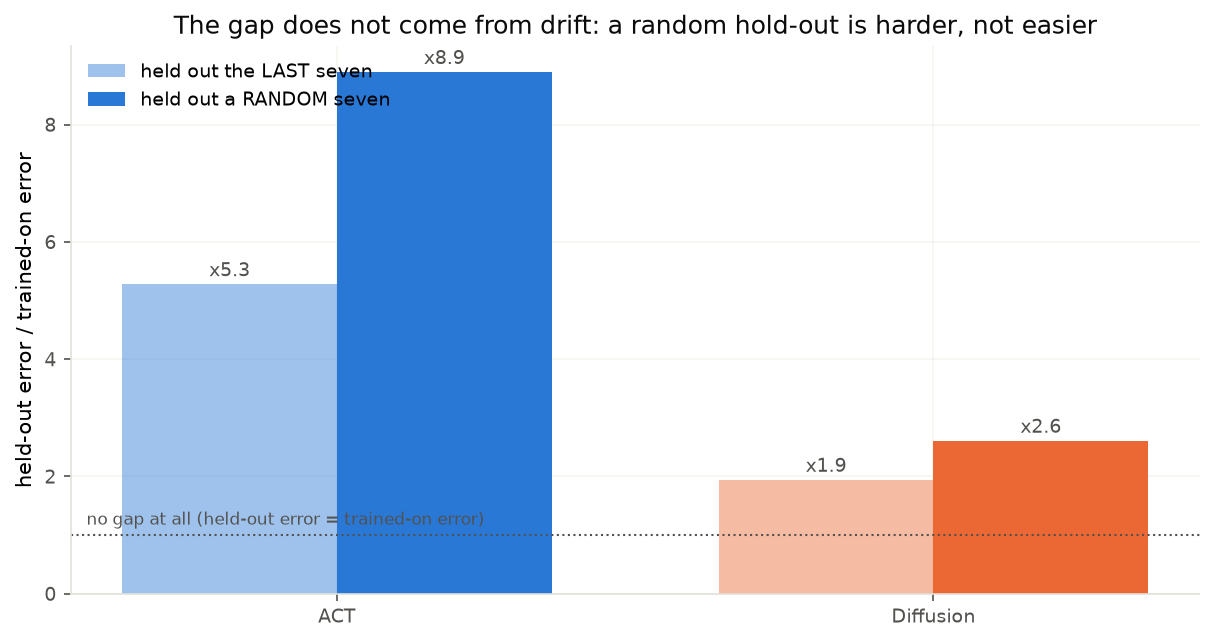
\includegraphics[width=0.45\textwidth]{split_comparison.png}
  \caption{The gap (test error divided by training error) when testing on the
  last seven demonstrations and on a random seven. The dotted line is a model
  equally good on both.}
  \label{fig:split}
\end{figure}

\begin{figure}[h]
  \centering
  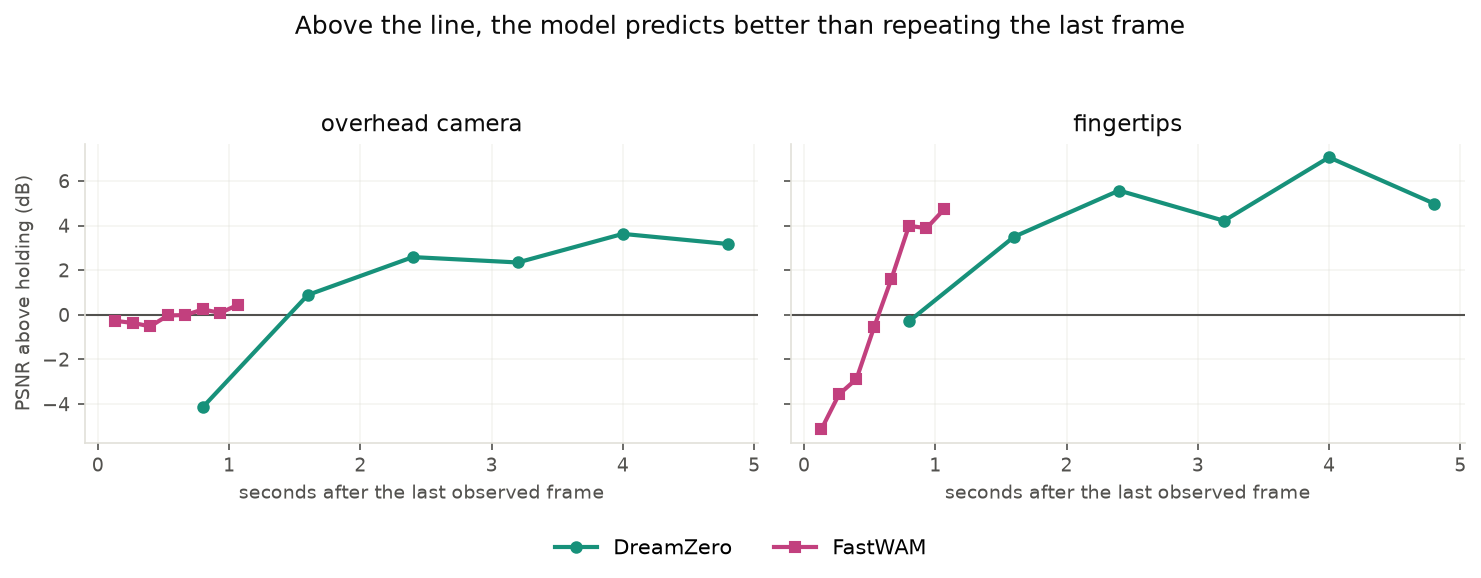
\includegraphics[width=0.8\textwidth]{prediction_margin.png}
  \caption{Each world action model's PSNR minus that of repeating the last
  frame, against how far ahead the frame is. Above zero, the model predicts
  better than assuming nothing moves.}
  \label{fig:predmargin}
\end{figure}



\begin{figure}[h]
  \centering
  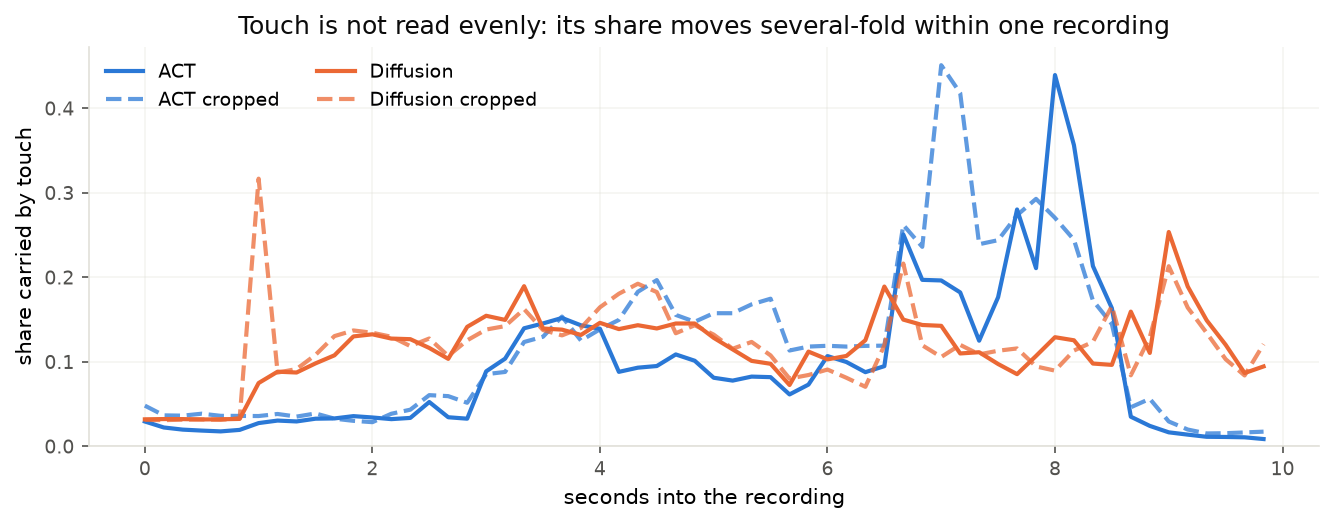
\includegraphics[width=0.68\textwidth]{framewise_shares.png}
  \caption{The fingertips' share of each policy's plan through one test
  demonstration. Dashed lines are the cropped versions.}
  \label{fig:framewise}
\end{figure}

\gn{\textbf{Touch matters only in short bursts around contact.} By a
\emph{burst} we mean a short stretch of a demonstration in which a model's plan
suddenly depends strongly on the fingertips, between longer stretches in which
it hardly depends on them at all.} Figure~\ref{fig:framewise} tracks the
fingertips' share through one test demonstration. For ACT it runs from under
1\,\% to 44\,\% within ten seconds, against an average of 10\,\%. It is nearly
ignored for the first three seconds and carries two fifths of the plan around
contact. An average therefore describes no moment that actually happens.
Diffusion and pi0.5 read touch more steadily, peaking at two to two and a half
times their own average where ACT peaks at four to five times.

\begin{table}[h]
  \centering
  \caption{The gap under each held-out set.}
  \label{tab:split}
  \small
  \begin{tabular}{lrrr}
    \toprule
    model & last seven & random seven & change \\
    \midrule
    ACT & 5.3 & 8.9 & $+68\,\%$ \\
    Diffusion & 1.9 & 2.6 & $+37\,\%$ \\
    \bottomrule
  \end{tabular}
\end{table}

Scoring each of the random seven on its own shows one atypical demonstration,
with nearly twice the median error of the other six. Without it, ACT's gap is
still 7.4, above the 5.3 of the last seven.

\begin{table}[h]
  \centering
  \caption{ACT with the rows-only crop, stretched and unstretched, over the
  first 10, first 32 and all 100 steps (test RMSE).}
  \label{tab:stretch}
  \small
  \begin{tabular}{lrrrr}
\toprule
& \multicolumn{3}{c}{held-out} & trained-on \\
\cmidrule(lr){2-4}\cmidrule(lr){5-5}
ACT arm & first 10 & first 32 & all 100 & all 100 \\
\midrule
not cropped & 7.88 & 10.11 & 14.09 & 2.67 \\
cropped and stretched back & 7.88 & 9.99 & 14.68 & 2.63 \\
cropped, not stretched & 7.58 & 9.56 & 14.08 & 2.59 \\
\bottomrule
\end{tabular}

\end{table}

\begin{figure}[h]
  \centering
  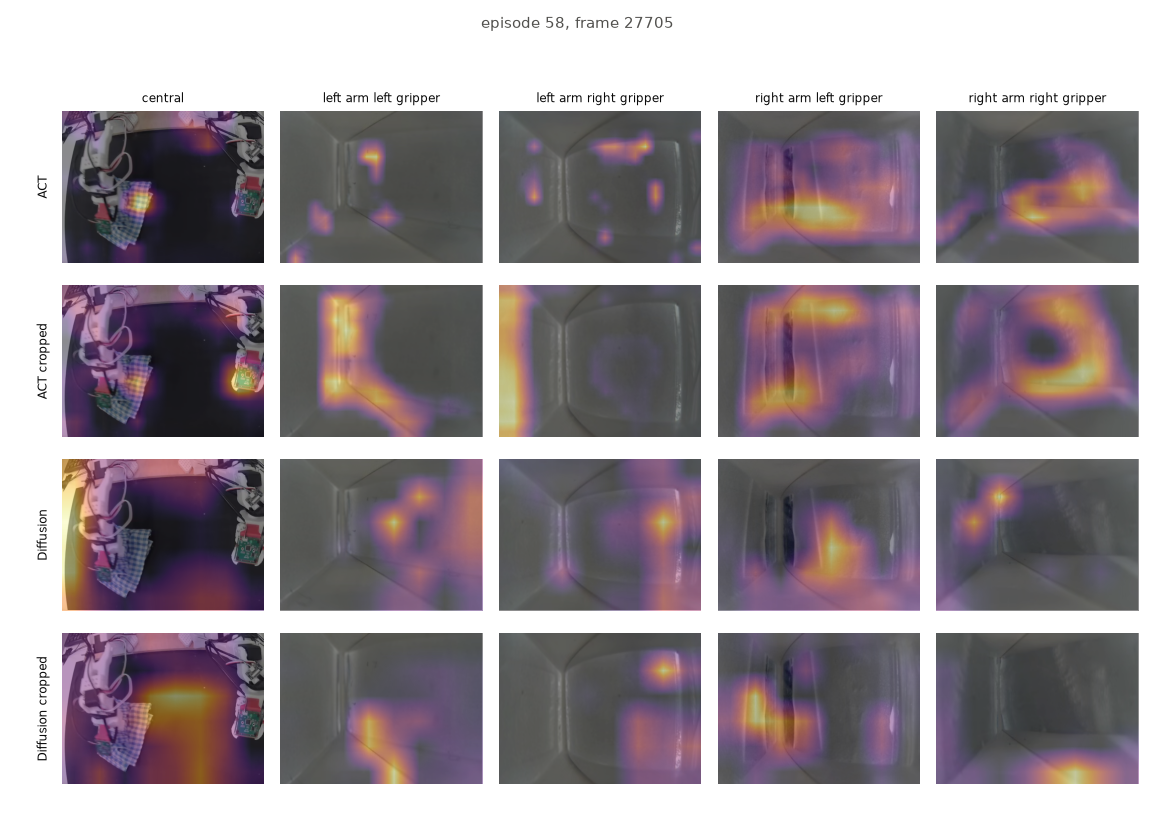
\includegraphics[width=\textwidth]{gradcam_peak_touch.png}
  \caption{Grad-CAM for each policy at the moment touch mattered most in test
  demonstration 58. A cropped policy is shown the cropped image it received.}
  \label{fig:gradcampeak}
\end{figure}

\begin{figure}[h]
  \centering
  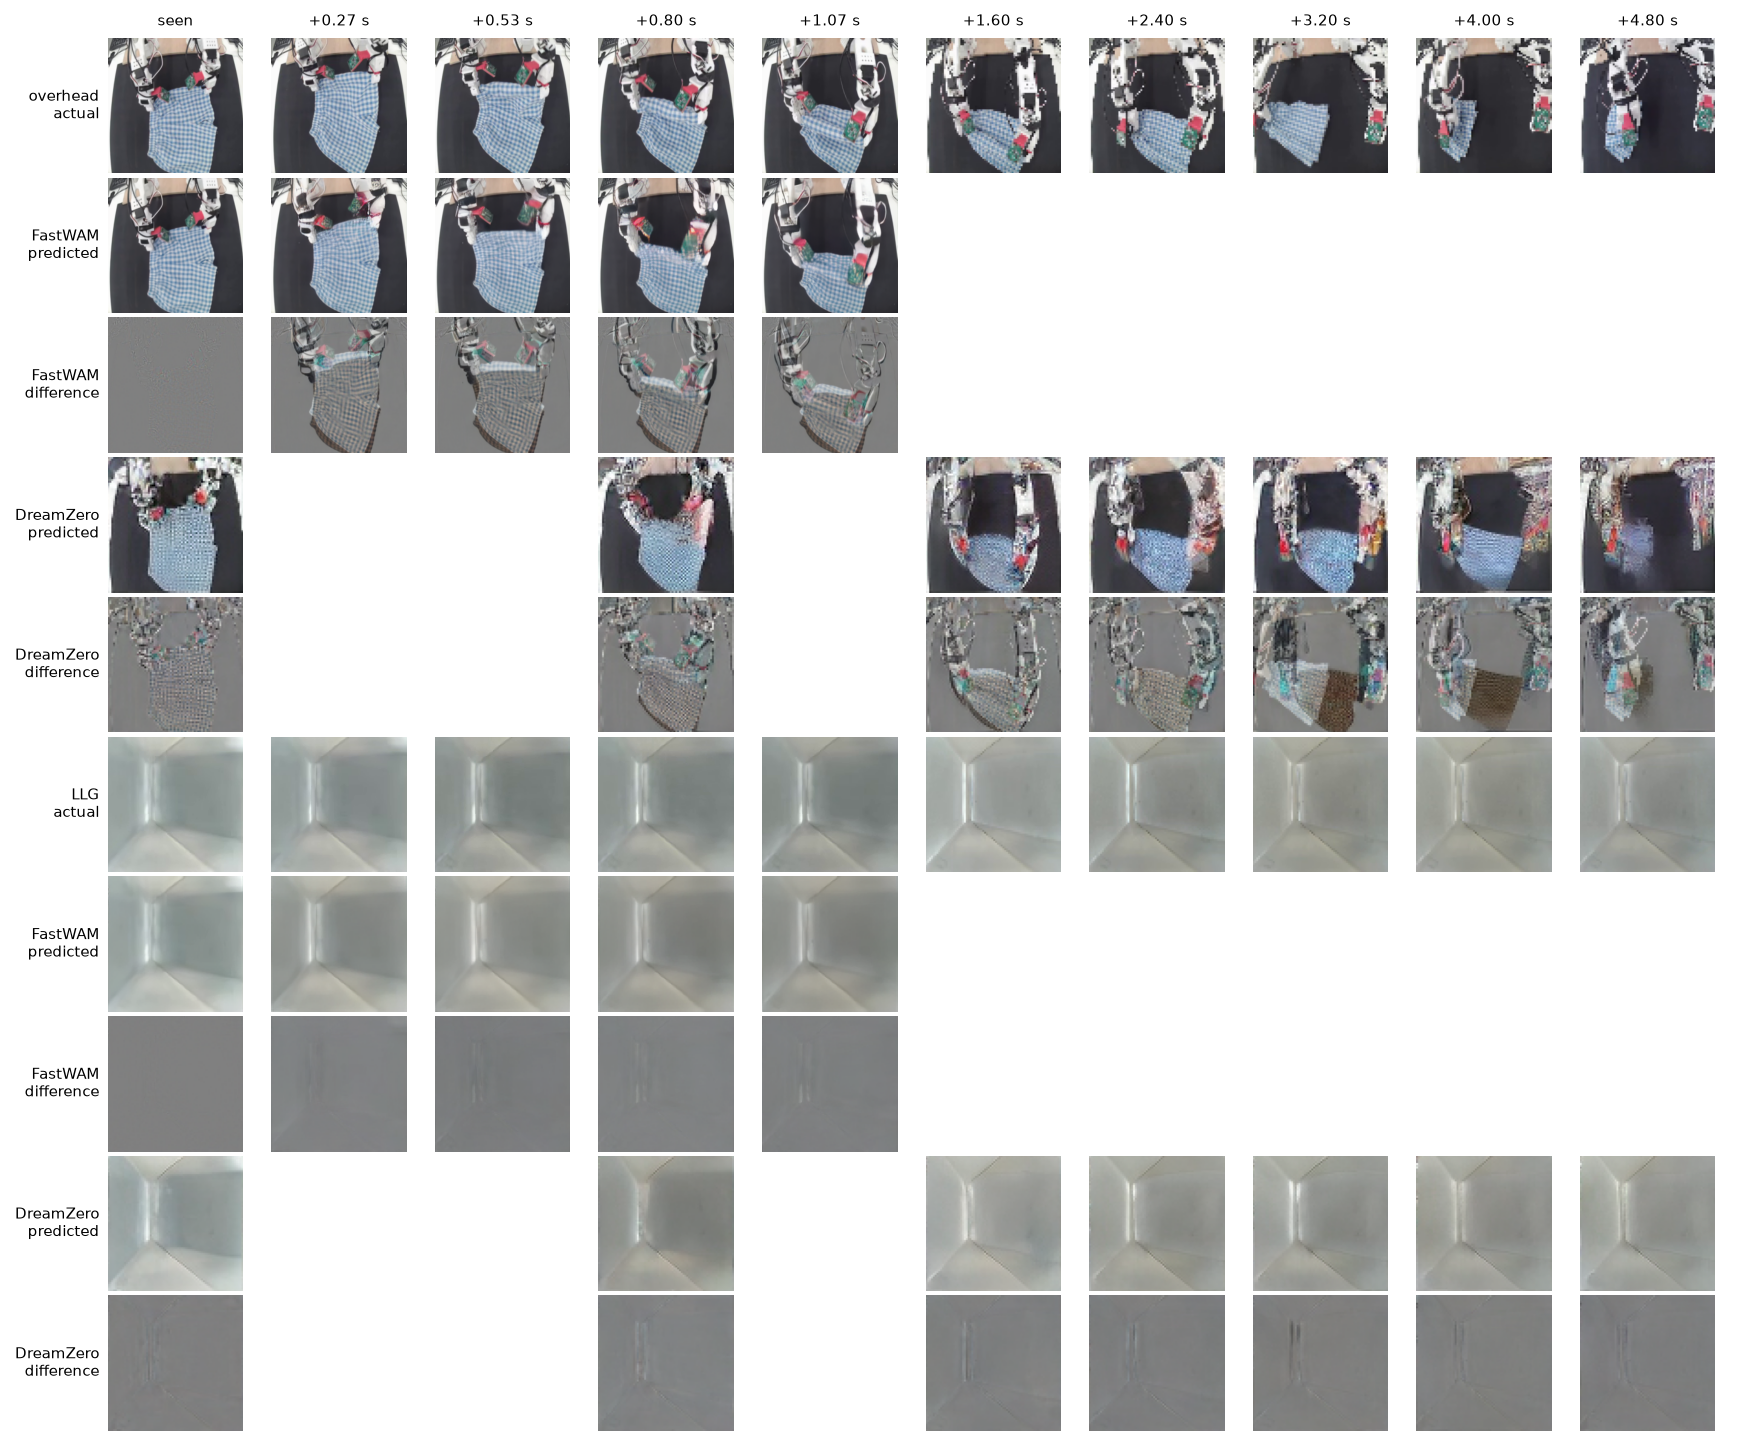
\includegraphics[width=\textwidth]{filmstrip_h2h_early.png}
  \caption{\new{As Figure~\ref{fig:filmstrip}, 4\,s into test demonstration
  58, as the arms lift the waistband. FastWAM moves the grippers but barely
  lifts the cloth; DreamZero predicts the fold, blurred and late.}}
  \label{fig:filmstripearly}
\end{figure}





















\gr{\begin{table}[h]
  \centering
  \caption{Input contribution (\%) of each model's inputs under the baseline of
  Figure~\ref{fig:streams} (images at their own mean colour, joints and past
  commands at their training mean) and under all zeros (black images, every
  joint and command at zero), on test demonstration 58. Each half of a row sums
  to 100 up to rounding; ``past'' is DreamZero's past commands.}
  \label{tab:baselines}
  \footnotesize
  \setlength{\tabcolsep}{4pt}
  \begin{tabular}{lrrrrrrrr}
\toprule
& \multicolumn{4}{c}{mean colour, training-mean joints} & \multicolumn{4}{c}{all zeros} \\
\cmidrule(lr){2-5}\cmidrule(lr){6-9}
model & joints & past & overhead & fingertips & joints & past & overhead & fingertips \\
\midrule
ACT & 17 & 0 & 69 & 14 & 23 & 0 & 65 & 13 \\
Diffusion & 69 & 0 & 13 & 19 & 74 & 0 & 11 & 15 \\
pi0.5 & 74 & 0 & 11 & 15 & 72 & 0 & 9 & 18 \\
Flow matching & 72 & 0 & 11 & 17 & 72 & 0 & 10 & 18 \\
DreamZero & 63 & 30 & 2 & 5 & 70 & 23 & 1 & 5 \\
FastWAM & 73 & 0 & 21 & 6 & 86 & 0 & 9 & 5 \\
\bottomrule
\end{tabular}

\end{table}}

\begin{thebibliography}{99}
\bibitem{gelsight} W.~Yuan, S.~Dong and E.~H. Adelson. GelSight: high-resolution
robot tactile sensors for estimating geometry and force. \emph{Sensors}, 17(12),
2017.
\bibitem{digit} M.~Lambeta et al. DIGIT: a novel design for a low-cost compact
high-resolution tactile sensor with application to in-hand manipulation.
\emph{IEEE RA-L}, 5(3), 2020.
\bibitem{bi2026vlatouch} J.~Bi, K.~Y. Ma, C.~Hao, M.~Z. Shou and H.~Soh.
VLA-Touch: enhancing vision-language-action models with dual-level tactile
feedback. \emph{IEEE RA-L}, 11(7):8487--8494, 2026.
\bibitem{helmut2026farm} E.~Helmut, N.~Funk, T.~Schneider, C.~de~Farias and
J.~Peters. Tactile-conditioned diffusion policy for force-aware robotic
manipulation. \emph{ICRA}, 2026.
\bibitem{heng2026vitacformer} L.~Heng, H.~Geng, K.~Zhang, P.~Abbeel and
J.~Malik. ViTacFormer: learning cross-modal representation for visuo-tactile
dexterous manipulation. \emph{RSS}, 2026.
\bibitem{higuera2025sparsh} C.~Higuera et al. Sparsh: self-supervised touch
representations for vision-based tactile sensing. \emph{CoRL}, PMLR
270:885--915, 2025.
\bibitem{higuera2025sparshx} C.~Higuera et al. Tactile beyond pixels:
multisensory touch representations for robot manipulation. \emph{CoRL}, PMLR
305:105--123, 2025.
\bibitem{huang2025vitac} B.~Huang, Y.~Wang, X.~Yang, Y.~Luo and Y.~Li. 3D-ViTac:
learning fine-grained manipulation with visuo-tactile sensing. \emph{CoRL}, PMLR
270:2557--2578, 2025.
\bibitem{li2026tacthru} Y.~Li, Y.~Chen, Z.~Zhao, P.~Li, T.~Liu, S.~Huang and
Y.~Zhu. Simultaneous tactile-visual perception for learning multimodal robot
manipulation. \emph{IEEE RA-L}, 11:5254--5261, 2026.
\bibitem{xue2025rdp} H.~Xue et al. Reactive diffusion policy: slow-fast
visual-tactile policy learning for contact-rich manipulation. \emph{RSS}, 2025.
\bibitem{zhao2025polytouch} J.~Zhao, N.~Kuppuswamy, S.~Feng, B.~Burchfiel and
E.~Adelson. PolyTouch: a robust multi-modal tactile sensor for contact-rich
manipulation using tactile-diffusion policies. \emph{ICRA}, 104--110, 2025.
\bibitem{zhu2025touchwild} X.~Zhu, B.~Huang and Y.~Li. Touch in the wild:
learning fine-grained manipulation with a portable visuo-tactile gripper.
\emph{NeurIPS}, 2025.
\bibitem{ye2025dreamtacvla} G.~Ye et al. Learning to feel the future:
DreamTacVLA for contact-rich manipulation. arXiv:2512.23864, 2025.
\bibitem{higuera2026vtwm} C.~Higuera, S.~Arnaud, B.~Boots, M.~Mukadam,
F.~R. Hogan and F.~Meier. Visuo-tactile world models. arXiv:2602.06001, 2026.
\bibitem{zheng2026omnivta} Y.~Zheng et al. OmniVTA: visuo-tactile world modeling
for contact-rich robotic manipulation. arXiv:2603.19201, 2026.
\bibitem{lou2026dreamtac} Y.~Lou et al. Dream-Tac: a unified tactile world action
model for contact-rich robot manipulation. arXiv:2606.08737, 2026.
\bibitem{zhao2023act} T.~Z. Zhao, V.~Kumar, S.~Levine and C.~Finn. Learning
fine-grained bimanual manipulation with low-cost hardware. \emph{RSS}, 2023.
\bibitem{chi2023diffusion} C.~Chi et al. Diffusion Policy: visuomotor policy
learning via action diffusion. \emph{RSS}, 2023.
\bibitem{pi05} Physical Intelligence. $\pi_{0.5}$: a vision-language-action
model with open-world generalization. 2025.
\bibitem{hu2022lora} E.~J. Hu et al. LoRA: low-rank adaptation of large
language models. \emph{ICLR}, 2022.
\bibitem{lipman2023flow} Y.~Lipman et al. Flow matching for generative
modeling. \emph{ICLR}, 2023.
\bibitem{dreamzero} S.~Ye et al. World action models are zero-shot policies.
arXiv:2602.15922, 2026.
\bibitem{kim2024openvla} M.~J. Kim et al. OpenVLA: an open-source
vision-language-action model. \emph{CoRL}, 2024.
\bibitem{biderman2024lora} D.~Biderman et al. LoRA learns less and forgets less.
\emph{TMLR}, 2024.
\bibitem{fastwam} T.~Yuan, Z.~Dong, Y.~Liu and H.~Zhao. Fast-WAM: do world
action models need test-time future imagination? arXiv:2603.16666, 2026.
\bibitem{wan2025} Wan Team. Wan: open and advanced large-scale video generative
models. arXiv:2503.20314, 2025.
\bibitem{selvaraju2017gradcam} R.~R. Selvaraju et al. Grad-CAM: visual
explanations from deep networks via gradient-based localization. \emph{ICCV},
2017.
\bibitem{bhirangi2021reskin} R.~Bhirangi, T.~Hellebrekers, C.~Majidi and
A.~Gupta. ReSkin: versatile, replaceable, lasting tactile skins. \emph{CoRL},
2021.
\bibitem{zhang2026tacvla} K.~Zhang, H.~Zhang et al. TacVLA: contact-aware
tactile fusion for robust vision-language-action manipulation.
arXiv:2603.12665, 2026.
\bibitem{wang2021wedge} S.~Wang, Y.~She, B.~Romero and E.~Adelson. GelSight
Wedge: measuring high-resolution 3D contact geometry with a compact robot
finger. \emph{ICRA}, 2021.
\bibitem{donlon2018gelslim} E.~Donlon, S.~Dong, M.~Liu, J.~Li, E.~Adelson and
A.~Rodriguez. GelSlim: a high-resolution, compact, robust, and calibrated
tactile-sensing finger. \emph{IROS}, 2018.
\bibitem{shimonomura2019review} K.~Shimonomura. Tactile image sensors employing
camera: a review. \emph{Sensors}, 19(18):3933, 2019.
\bibitem{lin2025lighttact} C.~Lin, B.~Huo, M.~Yu, E.~Ruppel, B.~Chen,
J.~Francis and D.~Zhao. LightTact: a visual-tactile fingertip sensor for
deformation-independent contact sensing. arXiv:2512.20591, 2025.
\bibitem{cottrell2026durable} F.~R. Cottrell, M.~H. Tippur and E.~H. Adelson. A
durable vision-based tactile fingertip for robotic manipulation.
arXiv:2608.24242, 2026.
\bibitem{ruan2026retacact} Ruan et al. ReTac-ACT: a state-gated vision-tactile
fusion transformer for precision assembly. arXiv:2603.09565, 2026.
\bibitem{hansen2022vtrl} J.~Hansen, F.~Hogan, D.~Rivkin, D.~Meger, M.~Jenkin
and G.~Dudek. Visuotactile-RL: learning multimodal manipulation policies with
deep reinforcement learning. \emph{ICRA}, 2022.
\bibitem{openpi} Physical Intelligence. openpi: open-source models and code for
vision-language-action models. https://github.com/Physical-Intelligence/openpi,
2025.
\end{thebibliography}


\end{document}
